\documentclass[12pt,article,oneside]{memoir}



\title{\bigskip \bigskip All that glitters is not gold }

%\author{Thomas Van Hoey 司馬智}

%\author{\Large \vspace{0.05in} \normalsize\emph{} \footnotesize \url{}\vspace*{0.2in} }

\author{\Large  \vspace{0.05in} \small \protect\\ \emph{} \footnotesize \protect\\  }

%\author{ ()}

\date{}



% LAY OUT
\usepackage{geometry}
\geometry{% siehe geometry.pdf (Figure 1)
	bottom=30mm,
	showframe=false, % For debugging: try true and see the layout frames
	margin=30mm,
	marginparsep=3mm,
	marginparwidth=20mm
}


%\usepackage{float} % % Extendes support for floating objects (tables, figures), adds the [H] placing option (\begin{figure}[H]) which palces it "Here" (without any doubt).


% MARGIN NOTES
%\usepackage{marginnote}


%linguistic packages
\usepackage{gb4e} %glosses and examples

%%%%BEGIN DOCUMENT %%%
\usepackage{amsthm}
\newtheorem{theorem}{Theorem}[section]
\newtheorem{lemma}{Lemma}[section]
\theoremstyle{definition}
\newtheorem{definition}{Definition}[section]
\newtheorem{corollary}{Corollary}[section]
\newtheorem{proposition}{Proposition}[section]
\theoremstyle{definition}
\newtheorem{example}{Example}[section]
\theoremstyle{definition}
\newtheorem{exercise}{Exercise}[section]
\theoremstyle{remark}
\newtheorem*{remark}{Remark}
\newtheorem*{solution}{Solution}
\begin{document}



\published{20/3/2018}

\maketitle


\begin{abstract}
\vspace*{-0.75in}\noindent \emph{Abstract:} This innovative study shows that literary Chinese ideophones in the
lexical field of LIGHT are highly dynamic in their polysemous semantic
structure as it developed through time. Four case studies demonstrate
that a levelled approach with attention to diachronic prototype
semantics reveal different aspects of the nature of ideophones and their
meanings: the meanings tend to be concentrated in prototypical bundles
with extensions to fuzzy edges. Different homophonous lexical items may
influence each other in terms of their semantic preference. Type and
token frequency effects influence the entrenchment of certain meanings.
Prototypicality is shown to be transient, from the semasiological
perspective as well as from the onomasiological perspective.
Furthermore, the four levels of Mental Spaces, Frames, ICMs or Domains,
and Image Schemas are unifiable into one bigger framework furthers a
comprehensive understanding of the semantics of LIGHT ideophones, but
can be expanded to other semantic fields as well.
Diachronic prototype semantics, ideophones, historical linguistics,
lexical semantics
\end{abstract}

\section{Introduction}\label{introduction}

In the last twenty to thirty years, scholarly attention for ideophones
and sound symbolism has slowly left the margins of linguistic study
(Joseph 1997) as multiple researchers of language-specific studies put
their findings together, resulting in conference proceedings like Sound
Symbolism (Hinton, Nichols \& Ohala 1994) and Ideophones (Voeltz \&
Kilian-Hatz 2001), in an attempt to readdress the Saussurean dictum of
the arbitrariness of the sign. While this study attempts to continue
this scholarly aspiration of discovering non-arbitrary elements in
language, it will show that there is much flexibility and dynamicity in
the meaning side of such sound-symbolic items, like ideophones.

This will be done by first briefly surveying the state of the field
(section 2.1), introducing a cognitive folk model of symbolic assemblies
consisting of {[}sound/writing/meaning{]} (section 2.2), and narrowing
down the scope to LIGHT ideophones based on phonaestheme research and
data this study inherited from a phonological pre-study (sections 2.3
and 2.4). Next, some methodological points will be made: first, how
three Cognitive Linguistic perspectives on the meaning of ideophones may
be unified into a four-level model inspired by recent advances in
Conceptual Metaphor Theory (section 3.1). Second, how diachronic
prototype semantics will further our understanding of the semantics of
LIGHT ideophones (section 3.2). These two perspectives essentially form
the research question (section 3.3) that drives this research: what does
a leveled approach with attention to polysemy and prototypicality reveal
about the nature of ideophones? The answer will be revealed in four
corpus-based case studies (section 4), after which some discussion with
the relevant literature will be made (section 5) and a conclusion
(section 6).

\section{The background for this
study}\label{the-background-for-this-study}

\subsection{A brief survey of the state of the field of ideophone
research}\label{a-brief-survey-of-the-state-of-the-field-of-ideophone-research}

Linguistic non-arbitrariness, sound symbolism, can be understood as a
direct iconic link between the phonological pole and the semantic pole
of a symbolic assembly, in Langackerian terms (Langacker 1987; 1988;
1991a; 2000; 1991b; 2008) . But what are ideophones? The earliest
definition follows Clement Doke: ``A vivid representation of an idea in
sound. A word, often onomatopoetic, which describes a predicate,
qualificative or adverb in respect to manner, colour, sound, smell,
action, state or intensity'' (Doke 1935:118). A more recent definition,
by Mark Dingemanse, defines them as ``marked words that depict sensory
imagery'' (Dingemanse 2011:25). While the former definition has the
advantage of being applicable to the language group it was found in
(Bantu languages), it lacked the cross-linguistic applicability
Dingemanse's definition attempts to provide. We accept Dingemanse's
definition as a cross-linguistic comparative concept (Haspelmath 2010a),
while at the same time recognizing the need for more language-specific
categorical description (Haspelmath 2007; 2010b). In terms of Chinese
(or Sinitic languages), an exact definition is still lacking, but
certain prominent features seem to exist in what is considered
ideophonic. Let us discuss these different markedness strategies.

From a morphological perspective, these words often display full
reduplication or partial reduplication, e.g.~汪汪
wang\textasciitilde{}wang `woof-woof', and 忐忑 tan\textasciitilde{}te
`perturbed, disturbed', traditionally described in terms of either
letters (respectively AA for full reduplication and AB for partial
reduplication) or in terms `reduplicative characters' (diezi 疊字),
`alliteration' (shuangsheng 雙聲), or `reduplicative rhyme' (dieyun
疊韻, as in the case of cuotuo 蹉跎 `wasting time'). It should also be
mentioned that Chinese perspectives on this issue usually place a large
emphasis on the so-called ABB construction, where a (seemingly) random
word collocates with an ideophone to create an even bigger ideophone,
such as liang-jingjing 亮晶晶 `glittering, sparkling' in Mandarin, or
kim-siaksiak 金爍爍 `golden' in Southern Min (Taiwanese). In more formal
treatments of Chinese phonology and morphology, the semantics and
pragmatics of these constructions are downplayed, as can be seen in a
recent reference grammar of Chinese (Huang \& Shi 2016), where virtually
no attention is devoted to the diachronic evolution that led to the
synchronic constructions that appear in Modern Chinese. However, it must
be admitted that morphologically there has been much research devoted to
this question, which can be built on in future research.

So, what other ways of markedness have been observed in ideophones?
Apart from phonological investigations of tone (Mok 2001; Chang 2009),
the field is still very young for Chinese languages. In many other
languages, however, the experiential nature of ideophones has been put
to the fore. For example, the multimodality of Quichua ideophones is
argued to be so important to the nature of the usage of this word
category that traditional dictionaries, let alone a simple glossing, are
unable to do their semantics and pragmatics justice (Nuckolls 1996;
2016; 2017). The multimodality in question refers to the accompanying
gesture, which appears quite naturally when they are `performed' in
spoken natural (non-elicited) language, without however being necessary
nor sufficient for the ideophone's semantics. In other words, there is a
high tendency for gesture and the ideophone to co-occur, but it need not
be that way.

Similarly, multimodal foregrounding can also be observed in Japanese
ideophones. Dingemanse \& Akita (2016) showed in their study of
earthquake victims interviewed by the Japanese television broadcasting
company NHK how apart from gesture, intonational foregrounding also
plays a huge role in the performance and markedness of ideophones. For
example, they observed deviations from the normal pitch range-ideophones
being spoken either with a higher or lower pitch than the rest of the
clause. Also extra intonational pauses seemed to separate the ideophone
from the clause, presumably to allow some time for the listener to
mentally simulate or experience the semantics conveyed by the ideophone
in this context. Other foregrounding mechanisms mentioned by Dingemanse
\& Akita in this study are phonational in nature, e.g.~the use of
breathy, creaky, whispering and even growling voice.

In summary, these morphological, gestural, intonational, and phonational
markedness seem to feature prominently in the categorization of lexemes
as ideophones. A recent development for Japanese and Korean ideophone
systems is attributing scores according to different parameters to
lexemes, in order to study their `canonicality' (Kwon 2015; 2017),
similar to how transitivity has been treated in the past (Thompson \&
Hopper 2001). However, an investigation into the applicability of these
criteria to Chinese ideophones has not been undertaken yet.

Now, after briefly sketching the state of the field, we must turn to the
current study object, which is diachronic in nature. It was necessary to
discuss the multimodality of ideophones in order to understand what is
lost when performing this kind of research: study of (contemporary)
synchronic linguistic data allows the researcher to gather material,
like video or even audio recordings, that might show how certain phrases
and constructions are marked in ways mentioned above. This is not
available in diachronic research. However, with Chinese we are in a
relatively good position-the availability of large historical corpora,
native traditions of lexicography, and a writing system that, even
through stages of reanalysis, contains much semantic information
beneficial for our understanding of ideophones and their development
through time. In our phonological analysis below, we will discuss the
case study of ideophones that are situated in the semantic domain of
LIGHT. There are two reasons for choosing this semantic domain, which
will have consequences for assumptions made in this research.

\subsection{A cognitive folk model}\label{a-cognitive-folk-model}

The first reason is rather coincidental in nature: a few weeks ago we
attended a musical concert titled xingguang yiyi 星光熠熠 `starlight
shining bright'. However, after an informal questionnaire, it turned out
that not everybody was able to read this 熠熠 out loud as yìyì {[}ji˥˩
ji˥˩{]}, but that some people faultily guessed the pronunciation of this
word was zhézhé {[}ʈʂɤ˦˥ ʈʂɤ˦˥{]}. It struck us as very revealing that
the people participating in this very informal study were able to
recognize this word yiyi 熠熠 as an ideophone, with the right semantics,
but that the entrenchment of its pronunciation was not of the same the
degree as its semantics. To us, it seemed further evidence of how
symbolic assemblies, as they were construed in Langacker's work on
Cognitive Grammar (Langacker 1987), with their phonological poles and
semantic poles, as the only three units by which language can be
analyzed perhaps do not account for the full system as it is experienced
in China. That is to say, for spoken language, this framework appears to
us as one of the best out there, with a strong explanatory power.
However, recently more voices have been calling out to also consider the
written language when discussing grammar (Iwasaki 2015). With respect to
Chinese, this integration has been argued for by e.g.~Packard
(2001:306), and with regards to Chinese and Japanese ideophones, it has
been argued by Lu (2006) that a better semiotic model should connect ,
and into a . Building on this model, we have shown before that it could
explain two different strata in the current ideophonic vocabulary of
Mandarin Chinese, with some ideophones being interpreted as more
literary, supported by the writing system, and others being more
colloquial without this support. Both groups, however, had the
morphophonological support (Van Hoey 2017). The assumption that we make
here, then, is that languages that do not have a tradition of writing,
are describable in terms of Langacker's symbolic assemblies, but that
for languages that do have a writing system, there might be an
integration effect, differing in degree per language (and perhaps even
per construction?). The cognitive semiotic model for Chinese (presented
in 1) follows Lu's characterization, but is simplified to capture its
essence. A curious note is that this model has a folk model in the idea
that Chinese characters are the combination of shape, sound and meaning
(Hanzi de `xing yin yi' 漢字的「形 音 義」).

\[[\frac{sound}{writing}|MEANING]\]

In this model, it is still assumed that there are symbolic assemblies
through which most linguistic phenomena can be explained. However,
instead of only one formal pole, it is split into a pole and a pole. The
adoption of this model allows us to discuss the different ideophones
according to their phonological form and written form, although
considerably more analysis will be devoted to the first.

\section{Phonaesthemes and the phonological
pre-study}\label{phonaesthemes-and-the-phonological-pre-study}

Let us return to the motivations behind our study of LIGHT ideophones in
Premodern Chinese. The second reason to do so, lies in the long
tradition investigations into phonaesthemes have had in the 20th
century. As Lockwood \& Dingemanse (2015) discuss, the English gl-
phonaestheme has a long history, capturing the attention of big figures
in linguistics like Leonard Bloomfield. However, we have not found more
in-depth analysis of this word cluster than in the works of Magnus
(2001). She categorizes the different semantic differences in gl-
phonaesthemes according to the manner of light perception (2-4).

\begin{exe}
    \ex \begin{xlist}
        \ex Reflected or indirect light\\
            glare, gleam, glim, glimmer, glint, glisten, glister,               glitter, gloaming, glow
        \ex Indirect use of the eyes\\
            glance, glaze, glimpse, glint
        \ex Reflecting surfaces\\
            glacé, glacier, glair, glare, glass, glaze, gloss
        \end{xlist}
\end{exe}

We believe that her work is valid, although it is hard to claim that we
are dealing with a real iconic mapping between and ; it has been argued
that the gl- derives from a Proto-Indo-European stem *GHEL `yellow'
(Thompson 2017), although this does not necessarily rule out an iconic
relation. What can be said, however, is that there is a network of
similar sounds that express related meanings, i.e.~phonaesthemes.
Taxonomies of sound symbolic phenomena subsume these phonaesthemes in
conventional sound symbolism (Hinton, Nichols \& Ohala 1994) or
diagrammatic relative arbitrary iconicity (Sidhu \& Pexman 2017). This
last classification highlights the nature of the iconicity relation in
examples (2-4): diagrammatic, as opposed to imagic. As Dingemanse (2012)
discusses through his usage of Peircean terminology, there is a
gradation (rather than clear dichotomy) from imagic iconicity, pure
onomatopoeia, e.g. `woof-woof', to diagrammatic iconicity, which depicts
more abstract domains (Van Hoey \& Lu, soon to be under review).

In the preceding paper that focused on the phonological relation of
literary Chinese ideophones situated in the semantic domain of LIGHT,
the same assumption was made, viz. the search for a clear sound symbolic
relationship between and must be abandoned, even before the data was to
be presented. What, however, did lie within reach, is a quest for
networks of formal features that are related to similar sets of
meanings. We will quickly discuss how this pre-study was conducted and
some of its relevant implications.

From our usage-based database and the comprehensive online dictionary
Handian 漢典 35 types of ideophones were collected, all with a
reduplicative or partial reduplicative morphology (the AA and AB-types
discussed above), and all depicting LIGHT in some way, e.g. (4-6).

\begin{exe}
    \ex 灼灼 zhuózhuó 'evident, brilliant, aglow, vivid and vibrant, brightly blazing, plain and patent'
    \ex 爍爍 shuòshuò 'flashing, flaring, effulgent, alight, rutilant; splendrous' 
    \ex 煇煇huīhuī 'fire-red, blazing brightly; splendid; brilliant'
\end{exe}

The single syllables of these ideophones were then reconstructed to
Middle Chinese and Old Chinese using Baxter and Sagart's systems (Baxter
1992; Sagart 1999; Baxter \& Sagart 2014; 2015), see Table 1. Based on
the Old Chinese reconstruction, some were categorized as belonging to
the same word family, a term for words that share the same root but have
different affixes (Sagart 1999; Baxter \& Sagart 2014). In our case, we
used Bybee's (1985; 2001) way of linking different stems using phonemes,
as is shown in Figure 1.

\begin{longtable}[]{@{}lll@{}}
\toprule
\begin{minipage}[b]{0.33\columnwidth}\raggedright\strut
Nucleus = e Coda = obstruent\strut
\end{minipage} & \begin{minipage}[b]{0.29\columnwidth}\raggedright\strut
Nucleus = ə Coda = nasal\strut
\end{minipage} & \begin{minipage}[b]{0.29\columnwidth}\raggedright\strut
Nucleus = a Coda = nasal\strut
\end{minipage}\tabularnewline
\midrule
\endhead
\begin{minipage}[t]{0.33\columnwidth}\raggedright\strut
\strut
\end{minipage} & \begin{minipage}[t]{0.29\columnwidth}\raggedright\strut
\strut
\end{minipage} & \begin{minipage}[t]{0.29\columnwidth}\raggedright\strut
\strut
\end{minipage}\tabularnewline
\begin{minipage}[t]{0.33\columnwidth}\raggedright\strut
\strut
\end{minipage} & \begin{minipage}[t]{0.29\columnwidth}\raggedright\strut
\strut
\end{minipage} & \begin{minipage}[t]{0.29\columnwidth}\raggedright\strut
\strut
\end{minipage}\tabularnewline
\begin{minipage}[t]{0.33\columnwidth}\raggedright\strut
\strut
\end{minipage} & \begin{minipage}[t]{0.29\columnwidth}\raggedright\strut
\strut
\end{minipage} & \begin{minipage}[t]{0.29\columnwidth}\raggedright\strut
\strut
\end{minipage}\tabularnewline
\bottomrule
\end{longtable}

TABLE Table 1: Reconstructions to Old and Middle Chinese

\begin{figure}

\includegraphics[width=5in]{ideos/bybee} \caption{Word families in Bybee's theories}\label{fig:bybee}
\end{figure}

The phonological analysis showed that rather than stating a direct,
imagic sound symbolism between certain phonemes and the semantic domain
of LIGHT, there seemed to be a slight negative correlation between
labials and glotals, and a positive tendency for coronal and dorsal
features, both obstruents and nasals. However, it was concluded that the
most important finding was that we are in fact dealing with small
networks of word families that were reanalyzed throughout history.
Furthermore, they seemed to mainly fall into two big and dynamic
prototypical clusters with fuzzy edges, at least according to their type
frequency. It does raise the question whether the same prototypicality
effects can be observed in their semantics, and their token frequencies.
Both of these issues will be explored in this paper.

\section{Data of the current study}\label{data-of-the-current-study}

As mentioned at the end of last section, we want to explore the notions
of prototypicality and token frequency effects in the diachronic
semantic development of LIGHT ideophones. Rather than aiming for a
superficial study of the whole semantic field, we have opted for more
fine-grained analyses of the data we inherited from the phonological
study. More specifically, we will only treat those ideophones that have
a schwa nucleus and obstruent coda in their Old Chinese reconstruction,
and focus mostly on their full reduplication forms-AA is the most
prototypical way of forming ideophones in Middle Chinese (and also Old
Chinese), as was shown earlier by Van Hoey (2015).

TABLE 2: Ideophone types used as material in this study

Let us then first turn to the types that will be investigated in this
study. Table 2 shows these data points. We have listed them with their
Chinese characters (traditional characters), their Hanyu pinyin
transcription into Modern Mandarin, the Taiwanese Ministry of Education
(MOE) Dictionary definition, and the corresponding definition in Kroll's
(2015) A student's dictionary of Classical and Medieval Chinese. It
should be noted that the 2nd century AD Shuowen jiezi 說文解字
``Explaining Graphs and Analyzing Characters'' native dictionary glosses
most of these characters (or words) (see Baxter \& Sagart 1998) as
either meaning LIGHT (guang ye 「光也」) or SHINING (zhao ye 「照也」),
with only occasionally mentioning the source of the LIGHT, e.g.
`lightning beam' (dianguang ye 「電光也」). The later 18th century
Kangxi Dictionary 康熙字典 uses almost the same explanation, so we have
not provided either in our discussion here. What can be learned from
these dictionary explanations is that these words are treated as
(near-)synonyms. However, below we will show that their meanings do
differ in their semantic preference or collocational habits. But first
we need to explain the methodology used in this study.

\section{Methodology and research
question}\label{methodology-and-research-question}

While it is certainly necessary to adopt a comparative concept for
ideophones, we should also try to come up with a certain definition of
the language-specific category (Haspelmath 2010a) of `ideophones'. For
comparative concepts, we follow Dingemanse's definition, as mentioned
above (section 2.1) For now, it falls outside the scope of this study to
come up with certain criteria (organized classically or prototypically)
for such a language-specific category of ideophones, but we believe they
should be proposed usage-based and form the bottom-up. That is why we
focus on different lexemes in this study, lexemes that were argued to be
ideophonic to the Chinese literati culture of ages past. Three possible
definitional frameworks to ideophones will be discussed in the section
below in an attempt to unify them through recent advances in Conceptual
Metaphor Theory. After this, we must turn to the theory of diachronic
prototype semantics, and how it will be of use in this study. Lastly,
the research question will be restated, with all this background
information.

\subsection{Unifying three Cognitive Linguistics definitional
frameworks}\label{unifying-three-cognitive-linguistics-definitional-frameworks}

The first Cognitive Linguistics-oriented framework for discussing the
semantics of ideophones is represented by Janis Nuckolls's ongoing
studies of Pastaza Quichua ideophones (Nuckolls 1996; 1999; 2001; 2010;
2014; Nuckolls et al. 2017). She uses IMAGE SCHEMAS as the main way of
representing an ideophone's most basic meaning. In the most recent work
referred to here, however, she revisits some of her case studies to
stress their dynamic and multimodal nature, e.g.~polang is shown to be
licensed by either a `glide across water' or `glide up to the surface of
the water' schemas. It is important to note that IMAGE SCHEMAS here
seems to be interpreted more according to Johnson's (2005) rich semantic
scenarios than the slightly more abstract usage found in most
discussions on the term (Hampe \& Grady 2005; Oakley 2007). That being
said, the difference between the two is only one of gradation.

A second framework is Lu Chiarung's 呂佳蓉 (2006) treatment of Japanese
(and Mandarin Chinese) mimetics or ideophones. Lu stresses the scenario
or script nature of ideophones and thus uses an IDEALIZED COGNITIVE
MODEL (ICM) (Lakoff 1987) approach. Her main examples are Japanese
korokoro コロコロ `(something small) rolling' and gorogoro ゴロゴロ
`(something large) rolling'. She shows that the dimensions of the
object, as well as the manner of movement etc. can be abstracted into an
ICM that could be used to define the meaning of these lexemes.

The third framework is represented by Akita Kimi 秋田喜美: FRAME
SEMANTICS. Akita argues that Japanese ideophones tend to be highly
specific in their semantics and invoke highly specialized frames, with
little semantic extension (Akita 2012). This is contrasted with the way
SOUND ideophones are depicted in Chinese, slightly vague and with many
possible referents (Akita 2013). However, as soon as we leave the imagic
iconicity of SOUND ideophones to more diagrammatic end of the iconicity
spectrum (Dingemanse 2012), it will become untenable to state that
Chinese ideophones are only vague, and not polysemous, as we will
illustrate with LIGHT ideophones.

The three frameworks briefly discussed above all agree on the
encyclopedic nature of ideophones, their multimodality, and their
foregrounding markedness. However, it is hard to say that any of these
analyses is `the right framework', because they all emphasize different
aspects of meaning description. IMAGE SCHEMAS try to capture the most
prototypical meaning (similar to Tyler \& Evans' (2003) notion of the
so-called PROTOSCENE for prepositions); FRAME SEMANTICS, conversely,
stress the high specificity of ideophones; ICMs occupy the middle ground
and are perhaps most flexible, but only because they are flexible by
nature.

However, maybe we do not have to choose. Kövecses's (2017) most recent
study proposes an analysis on different levels of metaphor: on the
lowest level there are MENTAL SPACES, which connect the metaphors online
(working memory) as the discourse happens dynamically. One level higher
there are FRAMES and DOMAINS. DOMAINS are ``not analogue, imagistic
patterns of experience but propositional in nature in a highly schematic
fashion'' (Kövecses 2017:325), while FRAMES elaborate particular aspects
of the domain matrix. They are all elaborations of the highly abstract
IMAGE SCHEMAS, which are directly meaningful preconceptual structures,
that are highly schematic Gestalts, consist of continuous analogue
patterns and have an internal structure consisting of only a few parts
(Kövecses 2017:324). Figure 2 below attempts to capture these different
levels of metaphor in a diagram.

HERE IS A FIGURE

Based on in-class discussions of ideophone-related research, it
increasingly appears possible to say that ideophones are very similar to
metaphor: both are cognitive abilities but are also very
culture-specific. This notion deserves further exploration, but
unfortunately it falls outside the scope of this study. However, future
research should devote considerable attention to it. For now, we will
assume that Kövecses fourfold level approach to metaphor can also be
used for ideophones. Furthermore, for our purposes, it seems that
DOMAINS can be thought of as Lu's ICMs. Let us keep this in mind as we
turn to the second idea that drives this research: diachronic prototype
semantics.

\subsection{Diachronic prototype
semantics}\label{diachronic-prototype-semantics}

One of the big themes that propelled the Cognitive Linguistics movement
is the attention it devotes to semantics. As the semanticist Dirk
Geeraerts explains, in this framework, ``language is seen as a
repository of world knowledge, a structured collection of meaningful
categories that help us deal with new experiences and store information
about old ones'' (Geeraerts 1997:8). Two crucial issues in this theory
of categorization are the notion of prototypicality and that of
polysemy. Prototypicality emerged from a series of experiments by
psycholinguist Eleanor Rosch (1975; 1975) as a theory of categorization
that opposed the traditional categorical definitions which required
necessary and sufficient conditions. Rather, it was shown that some
members of a lexical field are better representatives of it than others,
e.g.~the robin is the most prototypical BIRD in Anglo-Saxon culture,
because it has wings, feathers etc. On the other hand, penguins,
ostriches and the like are less typical representatives of BIRD. Now the
question that relates this very brief summary to our study is, can we
find the same prototypical structure in the semantics of LIGHT
ideophones?

This question presupposes that an ideophonic item is polysemous (the
second notion), i.e.~a series of interrelated meanings that are
activated according to the situation they are used in. Most Cognitive
Linguists appear to reject the idea that there is a single meaning for a
given lexical item (the monosemy hypothesis), instead opting for the
polysemy hypothesis. But if there is polysemy, how can we discern it
from vagueness? Useful discussions of the different approaches to the
phenomenon can be found in Tuggy (1993) and Geeraerts (2006a; 2010), to
name just two. Let us illustrate this with a classic example: fruit. In
a monosemous approach, such as the idealist Natural Semantic
Metalanguage developed by Wierzbicka (Wierzbicka 1992; Goddard \&
Wierzbicka 2014) they would give a definition built with so-called
semantic primes, concepts that exist in every language they have
developed the theory for. The idea is to get at the core experience or
core reasoning people use when they talk about fruit. Geeraerts, on the
other hand, does not agree with this and stresses the prototypical
polysemous structure of a word such as fruit. It is polysemous because
it has at least the meanings `something that people can eat and that
grows on a tree or a bush' and `the result or effect of something'.
However, it is also vague, with regard to the differences between
oranges and watermelons, because those differences do not lie at the
basis of a distinction between senses (Geeraerts 1997:18-19).

We have not gone in depth into the distinctions between the two
approaches (see for instance Geeraerts (2006b) for a detailed
discussion), but we think the polysemy with prototypicality is the more
interesting approach for this study. This is especially true in
Geeraerts's volume on diachronic prototype semantics, in which he
discusses the prototypical nature of the concept of `prototypicality'
itself (Geeraerts 1997:22), and some of the differences in semantic
changes that follow from it by stressing different parts of the concept.
We present it here in the revised version (Geeraerts 2010:189), in Table
3.

TABLE Extensional characterization (on the level of exemplars)
Intensional characterization (on the level of definition) Non-equality
(salience effects, core/periphery) (a) differences of typicality and
membership salience (b) clustering into family resemblances
Non-discreteness (demarcation problems, flexibility) (c) fuzziness at
the edges, membership uncertainty (d) absence of
necessary-and-sufficient definitions Table 3: Four types of
prototypicality effects

These four different types of prototypicality effects are put in a
diachronic perspective by Geeraerts (1997) and in a synchronic
perspective in Geeraerts (2010). Since our research is diachronic in
nature, we will follow the first of these two. As he relates (Geeraerts
1997: 23), the four effects are as follows (7-10):

\begin{exe}
    \ex By stressing the extensional non-equality of lexical-semantic structure, prototype theory highlights the fact that changes in the referential range of one specific word meaning may take the form of modulations on the core cases within that referential range.
    \ex By stressing the intensional non-equality of lexical-semantic structure, prototype theory highlights the clustered set structure of changes of word meaning.
    \ex By stressing the extensional non-discreteness of lexical-semantic structure, prototype theory highlights the phenomenon of incidental, transient changes of word meaning.
    \ex By stressing the intensional non-discreteness of lexical-semantic structure, prototype theory highlights the encyclopaedic nature of changes in word meaning.
\end{exe}

These four effects are all very interesting, but the one that is of most
interest to our current study is number 8. When this aspect of
prototypicality is stressed, the overall configuration of the various
readings of a word comes to the fore. This highlights two phenomena:
first, the overlapping and interlocking of the different readings, with
attention for the different starting points in existing meanings a novel
meaning may have. Second, the differences in structural weight among the
different meanings of an item. Some meanings do not survive very long,
other, more important (and prototypical) meanings persist through time.
Geeraerts (1997: 47-62) shows this through the analysis of the Dutch
verb ver-grijpen `mis-take'. After showcasing different meanings in
different historical contexts, he summarizes the data in a very nice
visualization, first shown in Geeraerts (1983), presented in Figure 3.

\begin{figure}
\centering
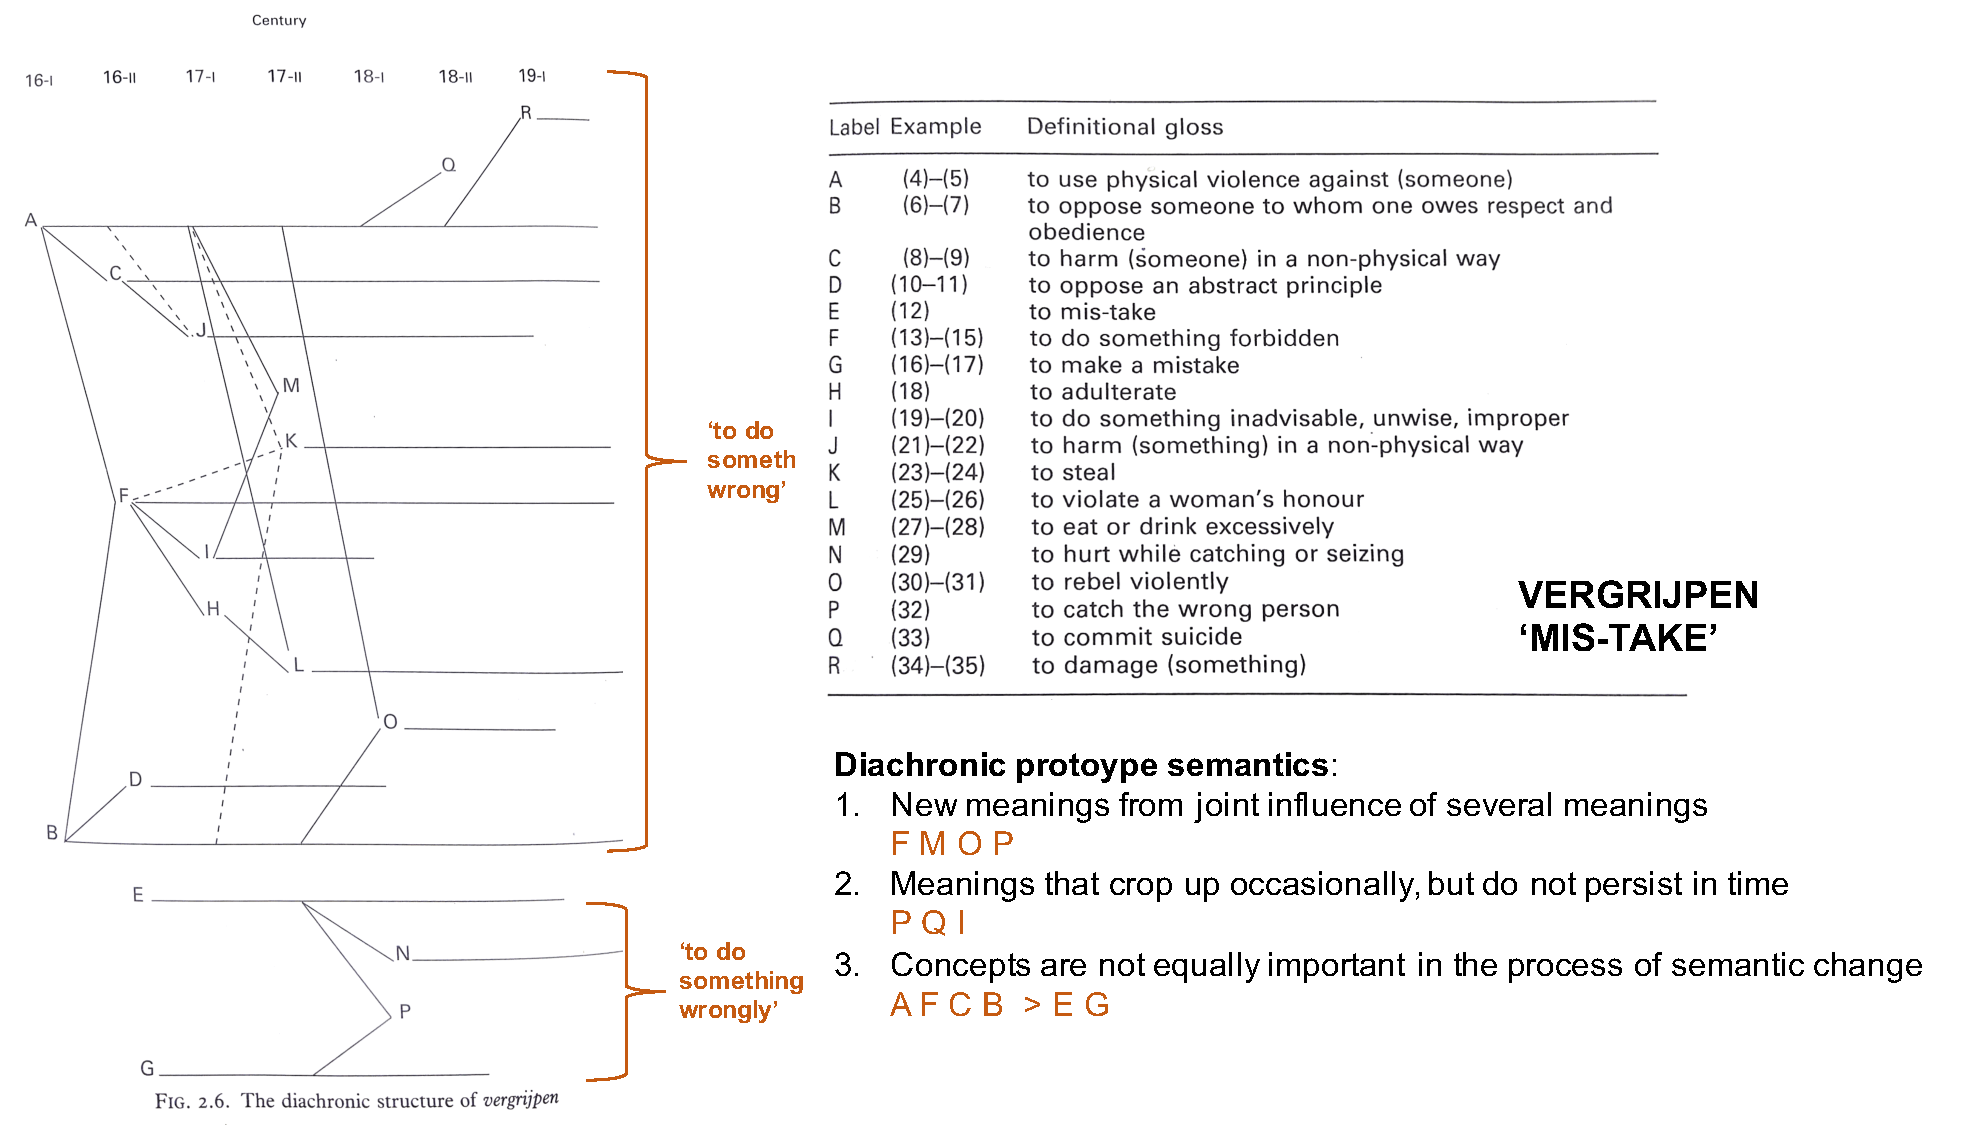
\includegraphics{ideos/vergrijpen.pdf}
\caption{\label{fig:levels}Vergrijpen}
\end{figure}

From the Figure above, we make three main observations. Firstly, new
meanings arise from the joint influence of several meanings,
e.g.~meaning F `to do something forbidden' has its conceptual starting
points in A `to use physical violence against (someone)', as well as B
`to oppose someone to whom one owes respect and obedience'. Secondly,
some meanings crop up occasionally, but do not persist in time, such as
Q `to commit suicide' can be seen as an extension of A, but it is used
in only one time period, 50 years in this case. Thirdly, not all
concepts are equally important in the process of semantic change. For
instance, A, B, C and F are more important than meanings E and G. This
diagram reveals much about the development of semantic structure, and we
will explore it further below.

\subsection{Research question}\label{research-question}

In general, it can be summarized from the preceding sections that a
diachronic analysis of ideophone semantic structure calls for a nuanced
leveled approach (section 3.1) with attention to prototype effects in
the polysemy of these items (section 3.2). We believe that such an
approach is innovative in many ways. For example, in section 2.4 we
showed that most dictionaries treat these LIGHT ideophones as
(near-)synonyms. However, as the case studies in section 4 will reveal,
this is far from their actual behaviour. So now we restate the research
question that drives this study: what does a leveled approach with
attention to polysemy and prototypicality reveal about the nature of
ideophones? Let us try to answer the question from different
perspectives in the case studies below.

\section{Mental spaces and Frames: corpus-based case
studies}\label{mental-spaces-and-frames-corpus-based-case-studies}

To study the items presented in Table 2 we made use of the very
comprehensive Scripta Sinica (Academia Sinica 中央研究院 2015) corpus.
For the present purpose, it must be noted that the corpus divides its
materials in periods of roughly 300 years, following the traditional
Chinese approach to historiography. In the visualizations below, we have
added a timeline to orient the reader who is not familiar with Chinese
dynastic history. This has two consequences: in comparison with
Geeraerts, it was not possible to do the same fine-grained analysis as
he did (periods of 50 years). On the other hand, it did make it possible
to see the bigger `macroevolutions' of the semantic networks. In the
context of the bigger Chinese historical corpus, the second evolution
seems the most interesting for the present.

It should also be mentioned that we tried to follow Tyler \& Evans'
(2003:38-45) methodology for determining different senses of the
different items, while trying to avoid the so-called `polysemy fallacy',
i.e.~positing more meanings than there actually are. In this regard, the
basic meaning of LIGHT may be maintained on the most abstract level of
image schemas but in the lowest level of mental spaces it is untenable,
as semantic preference (Geeraerts 2010:170-173) clearly demonstrates,
e.g.~yeye 曄曄 co-occurs mostly with plant-like meanings, as well as
light sources. This would count as at least two frames (a Plant frame
and a Lightsource frame), divided in many mental spaces. This will be
illustrated below clearer below.

Thirdly, one can wonder why a study on semantics is so lacking in
examples. This has a practical reason: we believe it is more important
now to focus on what the cases studies reveal than highlighting many
examples. However, the results were based on some 3500 tokens, which is
a decent number of examples to analyze manually. The distribution of
token frequency was not equal though, as e.g.~zhuozhuo 灼灼 was the most
frequently used ideophone in our dataset. See Figure 7 for a comparison
against three other ideophones.

Lastly, a methodological note: to consider a meaning as prototypical we
had three criteria that interplayed with each other: whether the meaning
persisted through time; whether it was productive for other meanings;
and whether it occurred in with high frequency. Given the unevenness in
the distribution, we have generally considered a tally of 5 occurrences
of a given meaning in a given period as `high frequency'. Of course,
compared to really frequent items, e.g.~closed-class items, this pales
in comparison. However, for ideophones it counts a high enough-bear in
mind that ideophones are presumed to be mostly performed in spoken
language, all we can work with in historical sources are the traces they
left behind in writings.

Let us now turn to the case studies, which all highlight a different
aspect of the prototypical and polysemic nature of LIGHT ideophones.

\subsection{Yueyue 爚爚}\label{yueyue-}

In the case of yueyue 爚爚, Figure 4 shows that there is a clear
prototypical core from its earliest occurrence, in the Qin-Han 秦漢
dynasties (ca. -221 BC - 220 AD). The main item yueyue describes is
LIGHTNING. At the same time, there is a meaning of SHOOT, which we
interpreted as a metaphor (`lightning fast'), although it is
speculation. Around the Tang dynasty, more LIGHT meanings develop,
related to the prototypical LIGHTNING: LIGHT (in general) and STARS.
From these onward there are usages that involve PEARLS and GOLD. There
is a large hiatus between the Yuan dynasty and the resurfacing usage of
LIGHT in the beginning of the 20th century. We presume LIGHT has taken
over the main prototypical core of yueyue and was still in use, but
unrecorded, until it resurfaced.

\begin{figure}
\centering
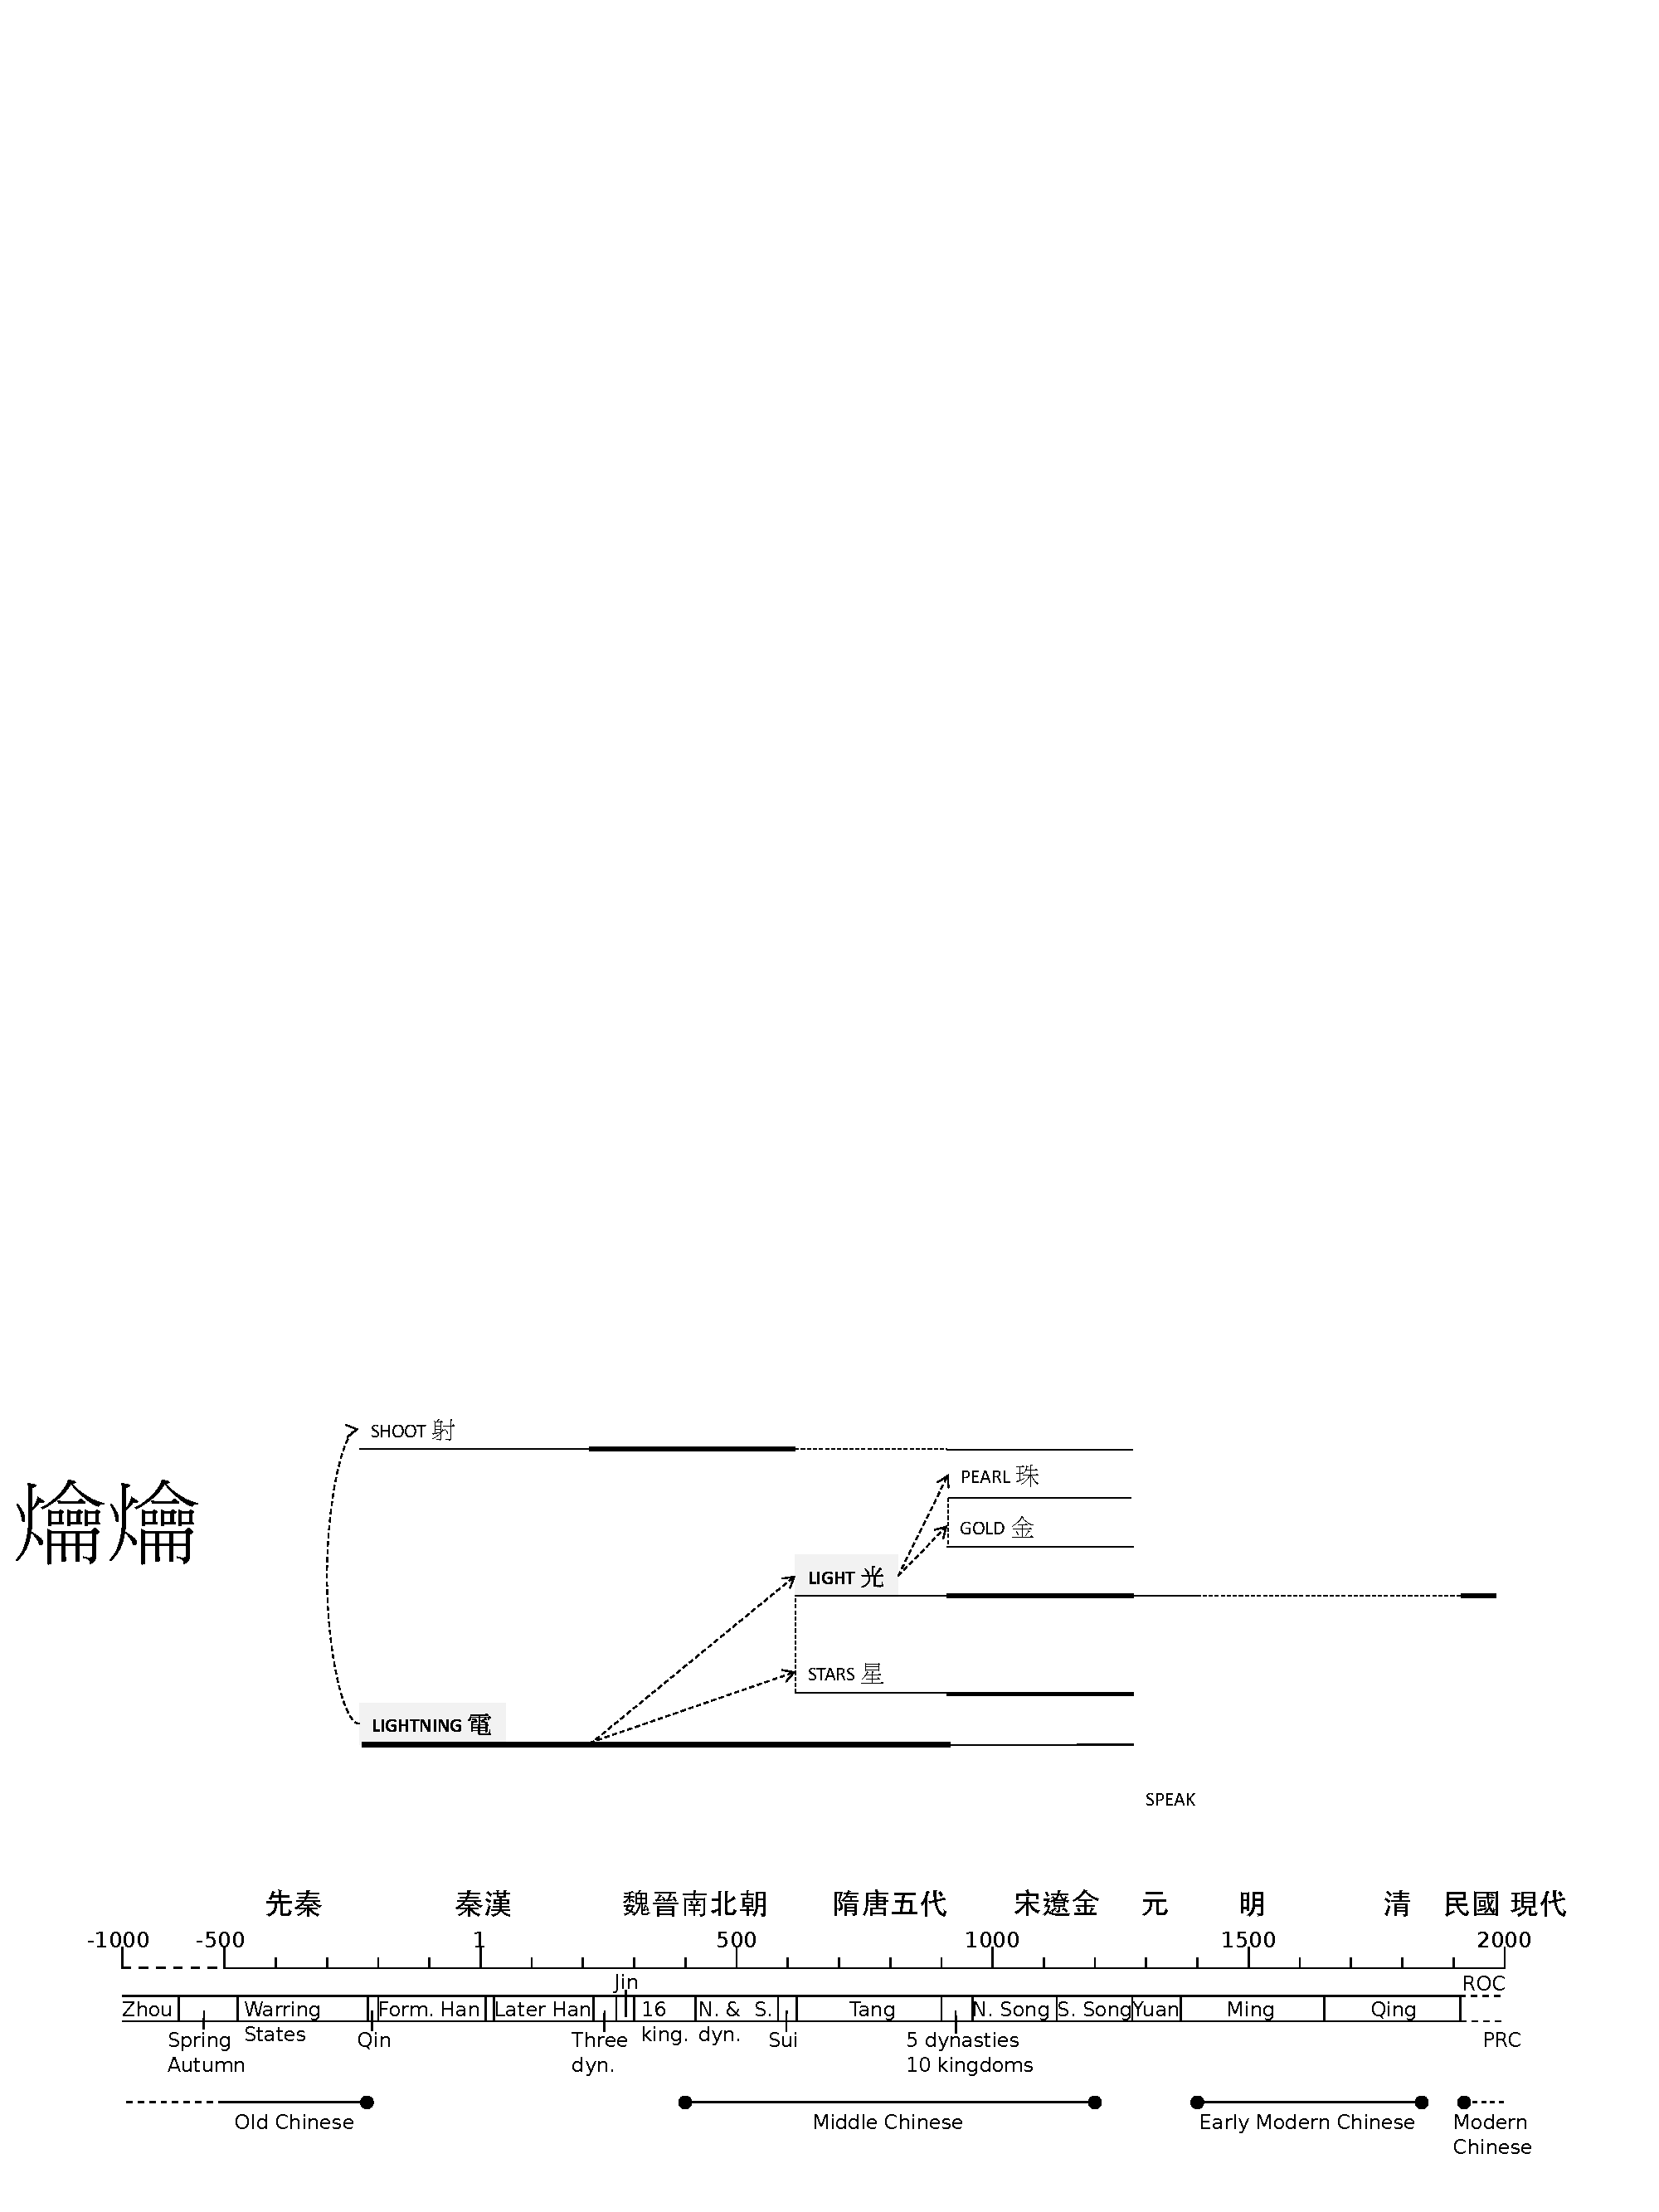
\includegraphics{ideos/yueyue.pdf}
\caption{\label{fig:yueyue}yueyue 爚爚}
\end{figure}

The visualization attempts to be improve upon Geeraerts's, shown above.
The difference in line thickness depict the higher and lower frequency.
The dotted lines indicate a presumed continuation of a certain meaning.
The dotted arrows are used to represent meaning extensions, following
Langacker's (2008:37) convention. Furthermore, in order to aid the
specialized reader that wants to perform the research him/herself, we
have included some of the more frequent collocations in Chinese next to
the meaning.

This case study of yueyue has shown how the visualizations should be
read and what can minimally be inferred from all of them. Let us move on
to the next case study.

\subsection{Yaoyao 燿燿 and yaoyao 耀耀}\label{yaoyao--and-yaoyao-}

The title of this case study shows that there is some variation in the
written form of yaoyao. The main difference is the radical that
distinguishes the two: either FIRE 火 or LIGHT 光. Does this
onomasiological (from meaning to form, as opposed to a semasiological
perspective, from form to meaning) difference show up in the usage of
these two items? In fact, it does. As Figure 5 clearly shows, yaoyaoFIRE
has an early usage of depicting LIGHTNING. This meaning is later picked
by in yaoyaoLIGHT during the Tang dynasty. Conversely, yaoyaoLIGHT has a
metaphorical extension to describe the POSTURE (of women) as `radiant,
shining', which finds its way in the meaning matrix yaoyaoFIRE. This
curious exchange of meanings shows the mutual influence related
semantics and a related phonological form may have on each other.

\begin{figure}
\centering
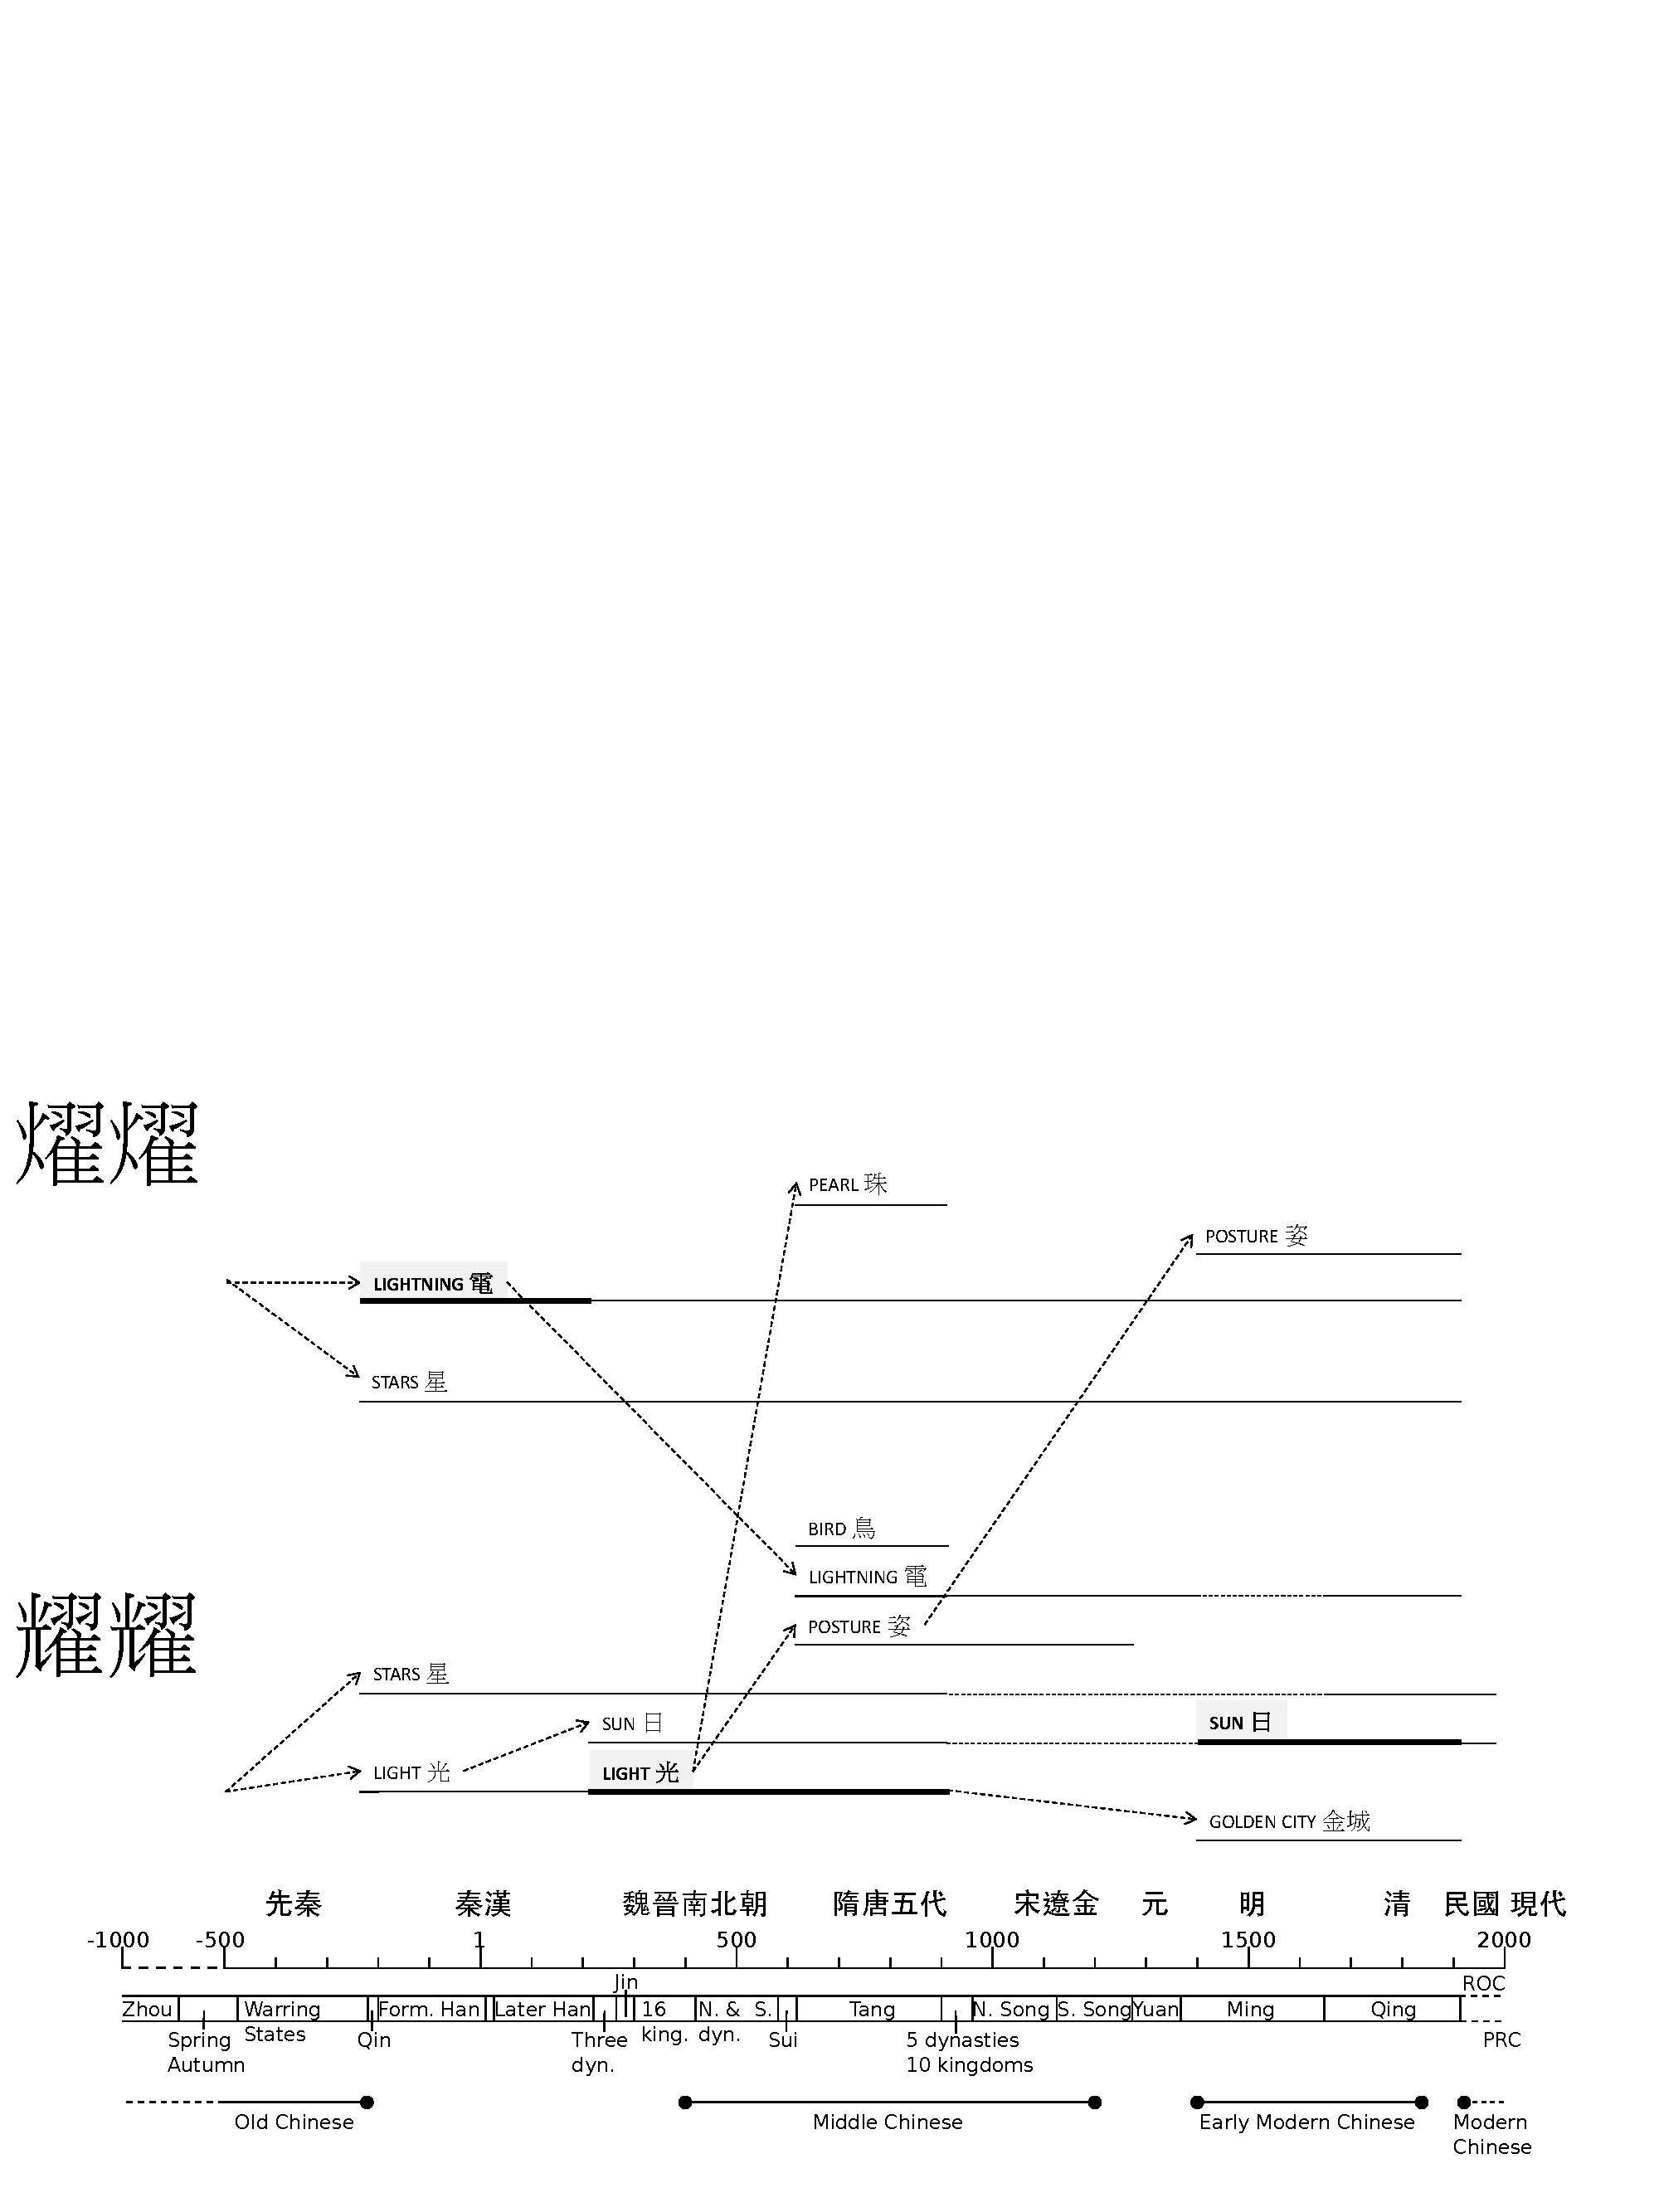
\includegraphics{ideos/yaoyao.pdf}
\caption{\label{fig:yaoyao}yaoyao 燿燿 and yaoyao 耀耀}
\end{figure}

\subsection{Huihui 煇煇, huihui 輝輝 and huihui 暉暉, vs.~zhuozhuo
灼灼}\label{huihui--huihui--and-huihui--vs.zhuozhuo-}

The next ideophonic trio displays similar effects as the two yaoyaos
discussed above: huihuiFIRE, huihuiLIGHT and huihuiSUN also mutually
influence each other. However, there is more going on. In Figure 6 it
can be seen that the meanings of huihuiFIRE and huihuiSUN are fewer in
number than those of huihuiLIGHT. All three, however, have their own
special usage, with e.g.~huihuiFIRE used mostly for LIGHTNING, but also
in a Chinese traditional medicinal context of DEAFNESS. What binds these
three together is their ability to depict different kinds of light, as
well as shades of RED.

\begin{figure}
\centering
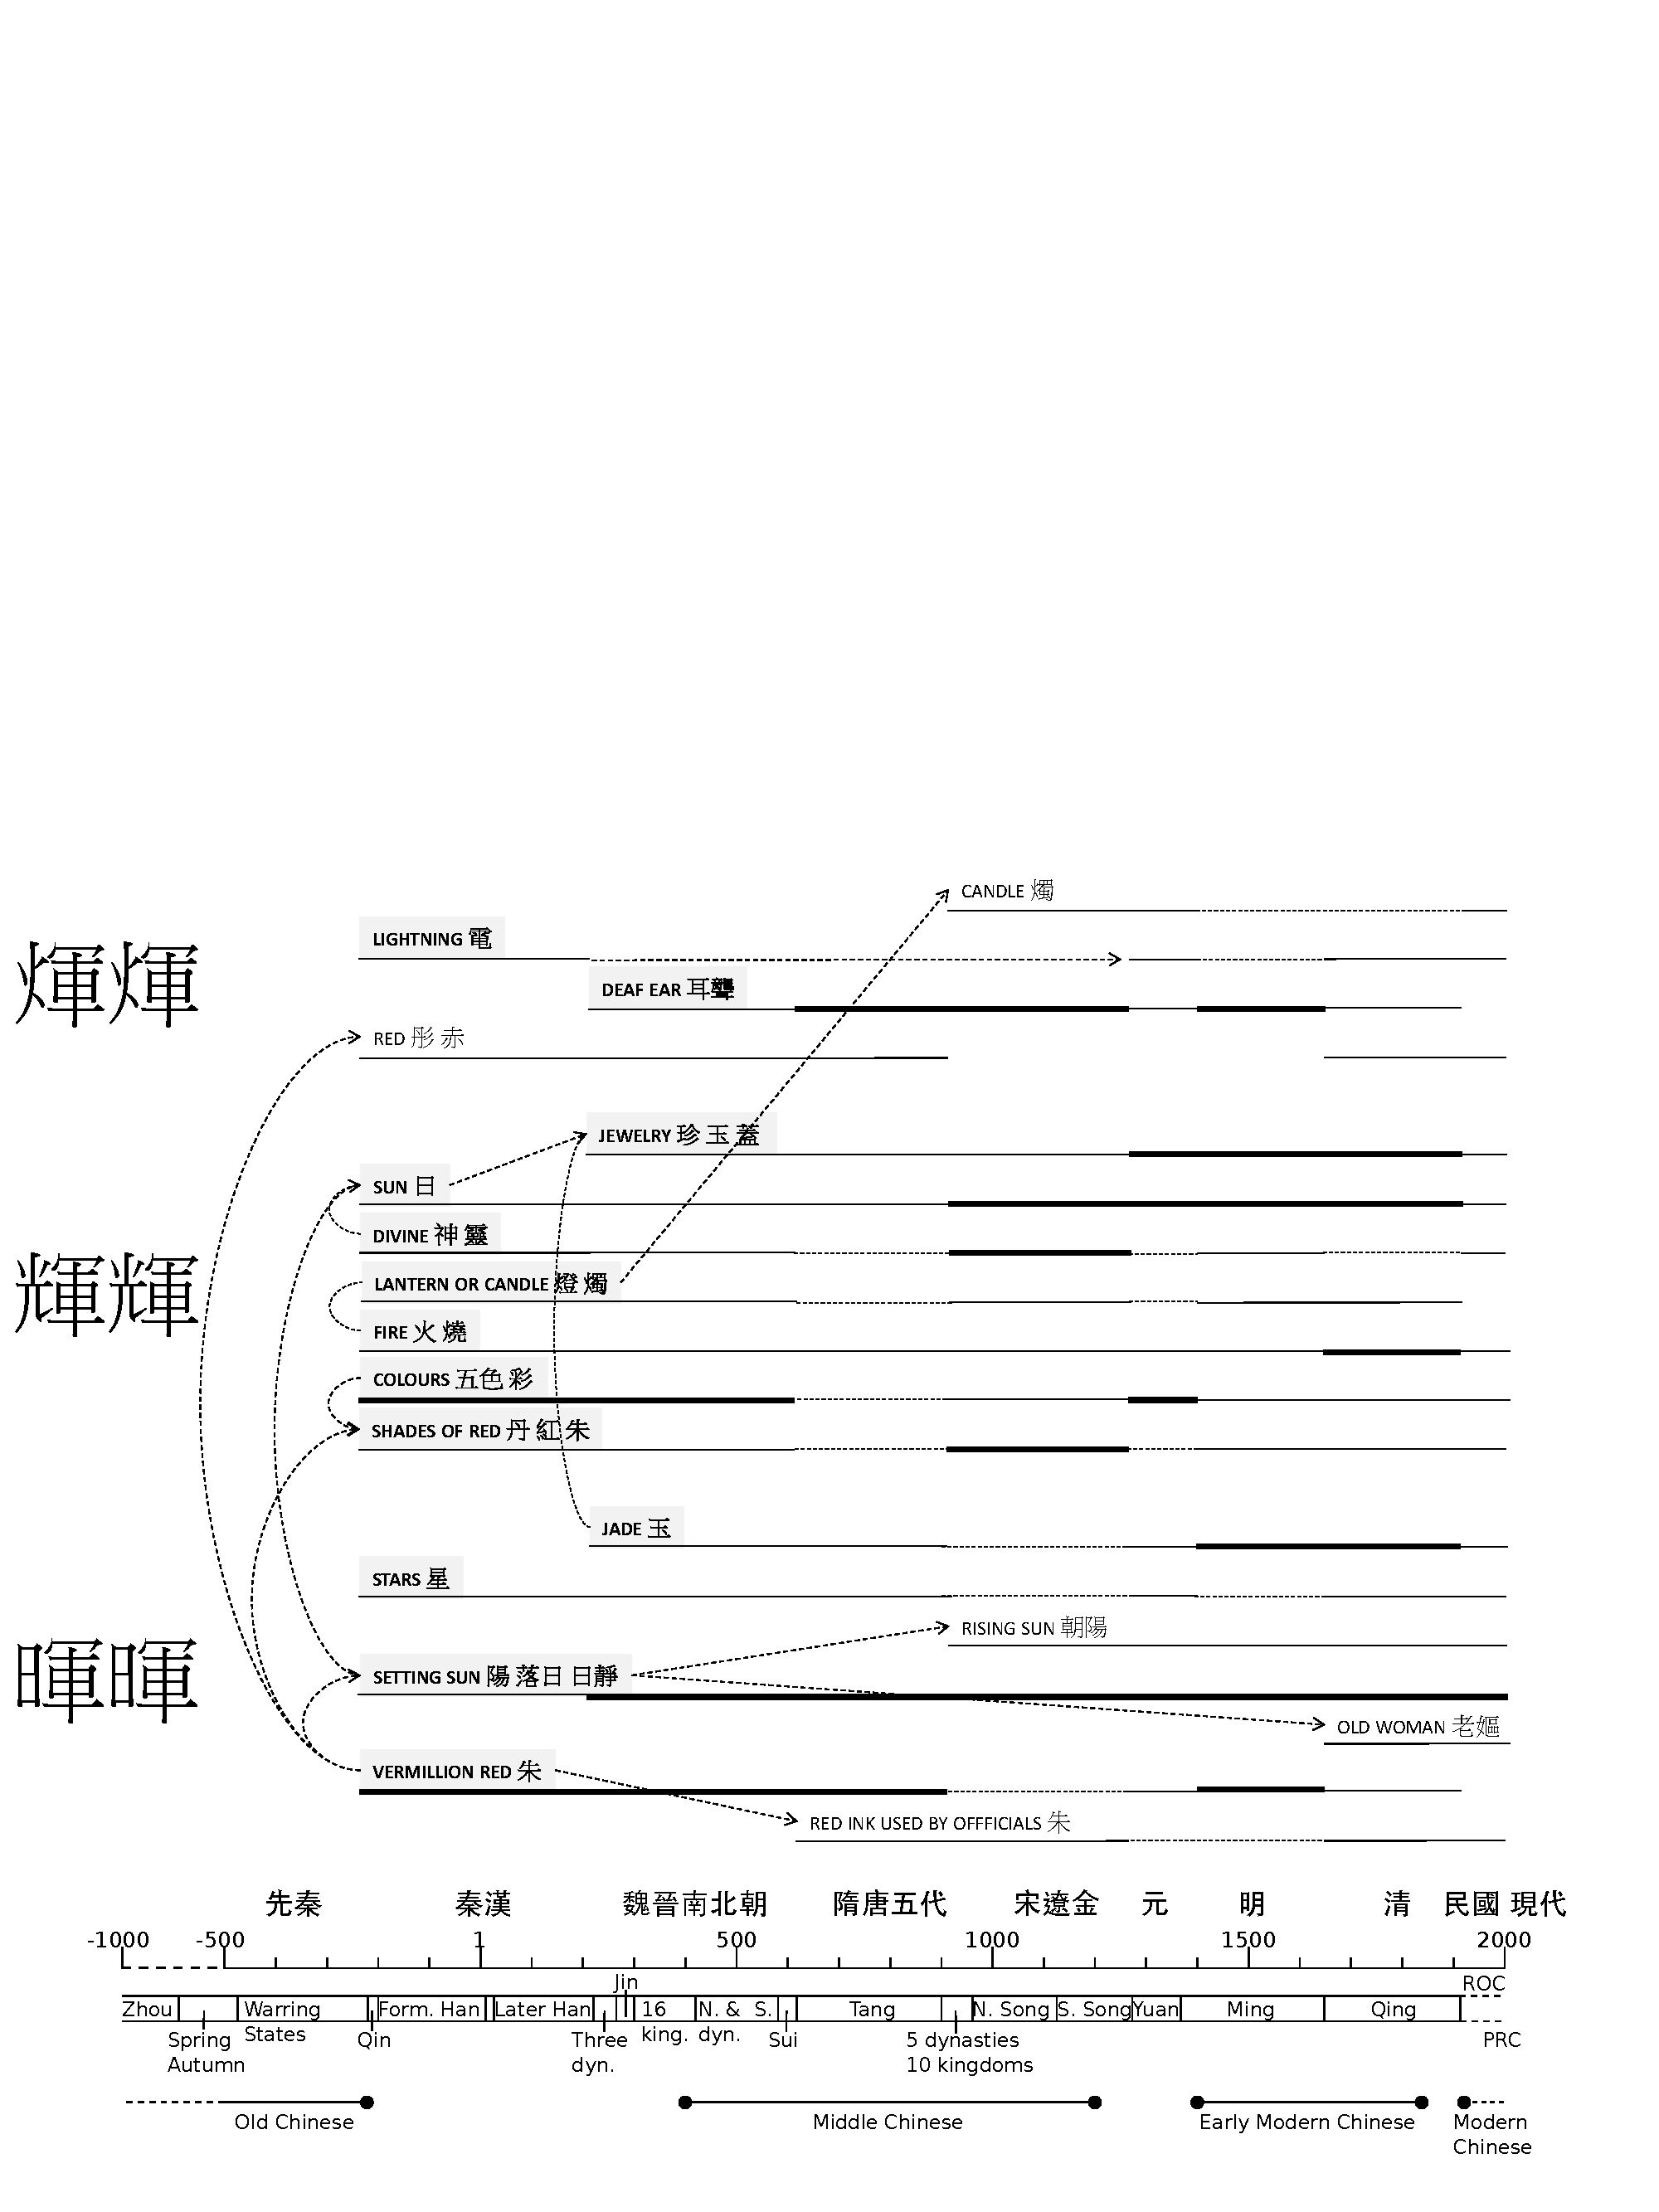
\includegraphics{ideos/huihui.pdf}
\caption{\label{fig:huihui}huihui 煇煇, huihui 輝輝 and huihui 暉暉}
\end{figure}

Now, this interplay between the three items is asymmetrical in a way,
precisely because huihuiLIGHT has the most productive set of
interrelated meanings. It has a higher type frequency, the effect of
which is the reinforcement of its productivity, similar to the English
past-tense suffix -ed (Bybee 2001). This polysemy was already found in
the earliest period the ideophones were encountered. We can only assume
that they were extended from even earlier meanings. That being said,
does this high type frequency also translate into high token frequency?
Figure 7 below shows that it clearly does, especially during the latter
half of the Chinese empirical history.

The effect of this high token frequency for huihuiLIGHT entrenches
certain meanings the more it is used. Let us take another ideophone,
zhuozhuo 灼灼, as a standalone example of how token frequency cements
certain meanings, and leaves dynamic usage for other ones. It should be
noted that zhuozhuo was the ideophone with the highest token frequency
throughout history, as can be seen in Figure 7 as well.

\begin{figure}
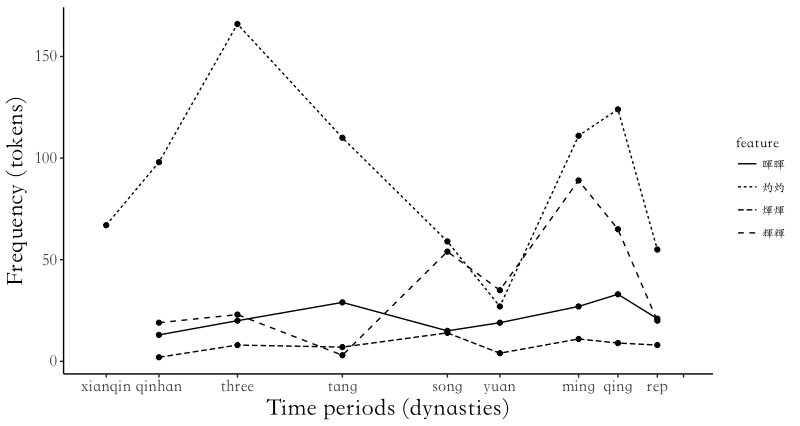
\includegraphics[width=11.11in]{ideos/huihuizhuozhuo} \caption{token frequencies of huihui and zhuozhuo}\label{fig:huizhuo}
\end{figure}

The meaning matrix of zhuozhuo revolves mostly around the shining
brilliance of things associated with spring and the blossoming of FLOWER
LEAVES, PINKISH RED and PEACH TREES. This extends to depict the dazzling
colours of CHRYSTANTHEMUMS, but also to `normal LIGHT' items. Another
extension from the prototypical bundle is that to the concept of
DENSENESS OF PLANTS. There is also a seemingly anomalous usage of
zhuozhuo to depict turtle(shells?), which we were not able to
convincingly relate to any of the other meanings.

What can be summarized from this exploration of the three huihuis and
zhuozhuo is that type frequency as well as token frequency certainly
have observable effects in the semantic structure of these items.

\subsection{Yeye 爗爗, yeye 燁燁 and yeye
曄曄}\label{yeye--yeye--and-yeye-}

The last case study, presented in Figure 7, shows the development of
yeyeFIRE+SUN, yeyeFIRE and yeyeSUN. It highlights two important features
of applying diachronic prototype semantics to LIGHT ideophones. First,
it is shown once more that the meanings (semantic preferences) of these
ideophones are dynamic, and are made in a case-to-case basis, which is
exactly what mental space theory suggests. They are also mediated by the
slightly more abstract frame theory, which in a way acts as a
highly-specialized repository of patterns.

Secondly, there is a shifting or transient prototypicality in these
items, from two perspectives. Semasiologically (from form to meaning),
this is expressed again in the different meanings that are more
prevalent during a certain period. Onomasiologically (from meaning to
form), yeyeSUN is the most productive in the former half of the Chinese
empirical history, but this role is taken over by yeyeFIRE in the latter
half. The complex written form of yeyeFIRE+SUN probably also influenced
its sporadic usage throughout time-there was already a form with FIRE
and a form with SUN that were both quite productive, so there was not
really a need for the complex FIRE+SUN grapheme in order to replace one
or the other (although a merge between the FIRE form and the SUN form
might have happened!).

\begin{figure}
\centering
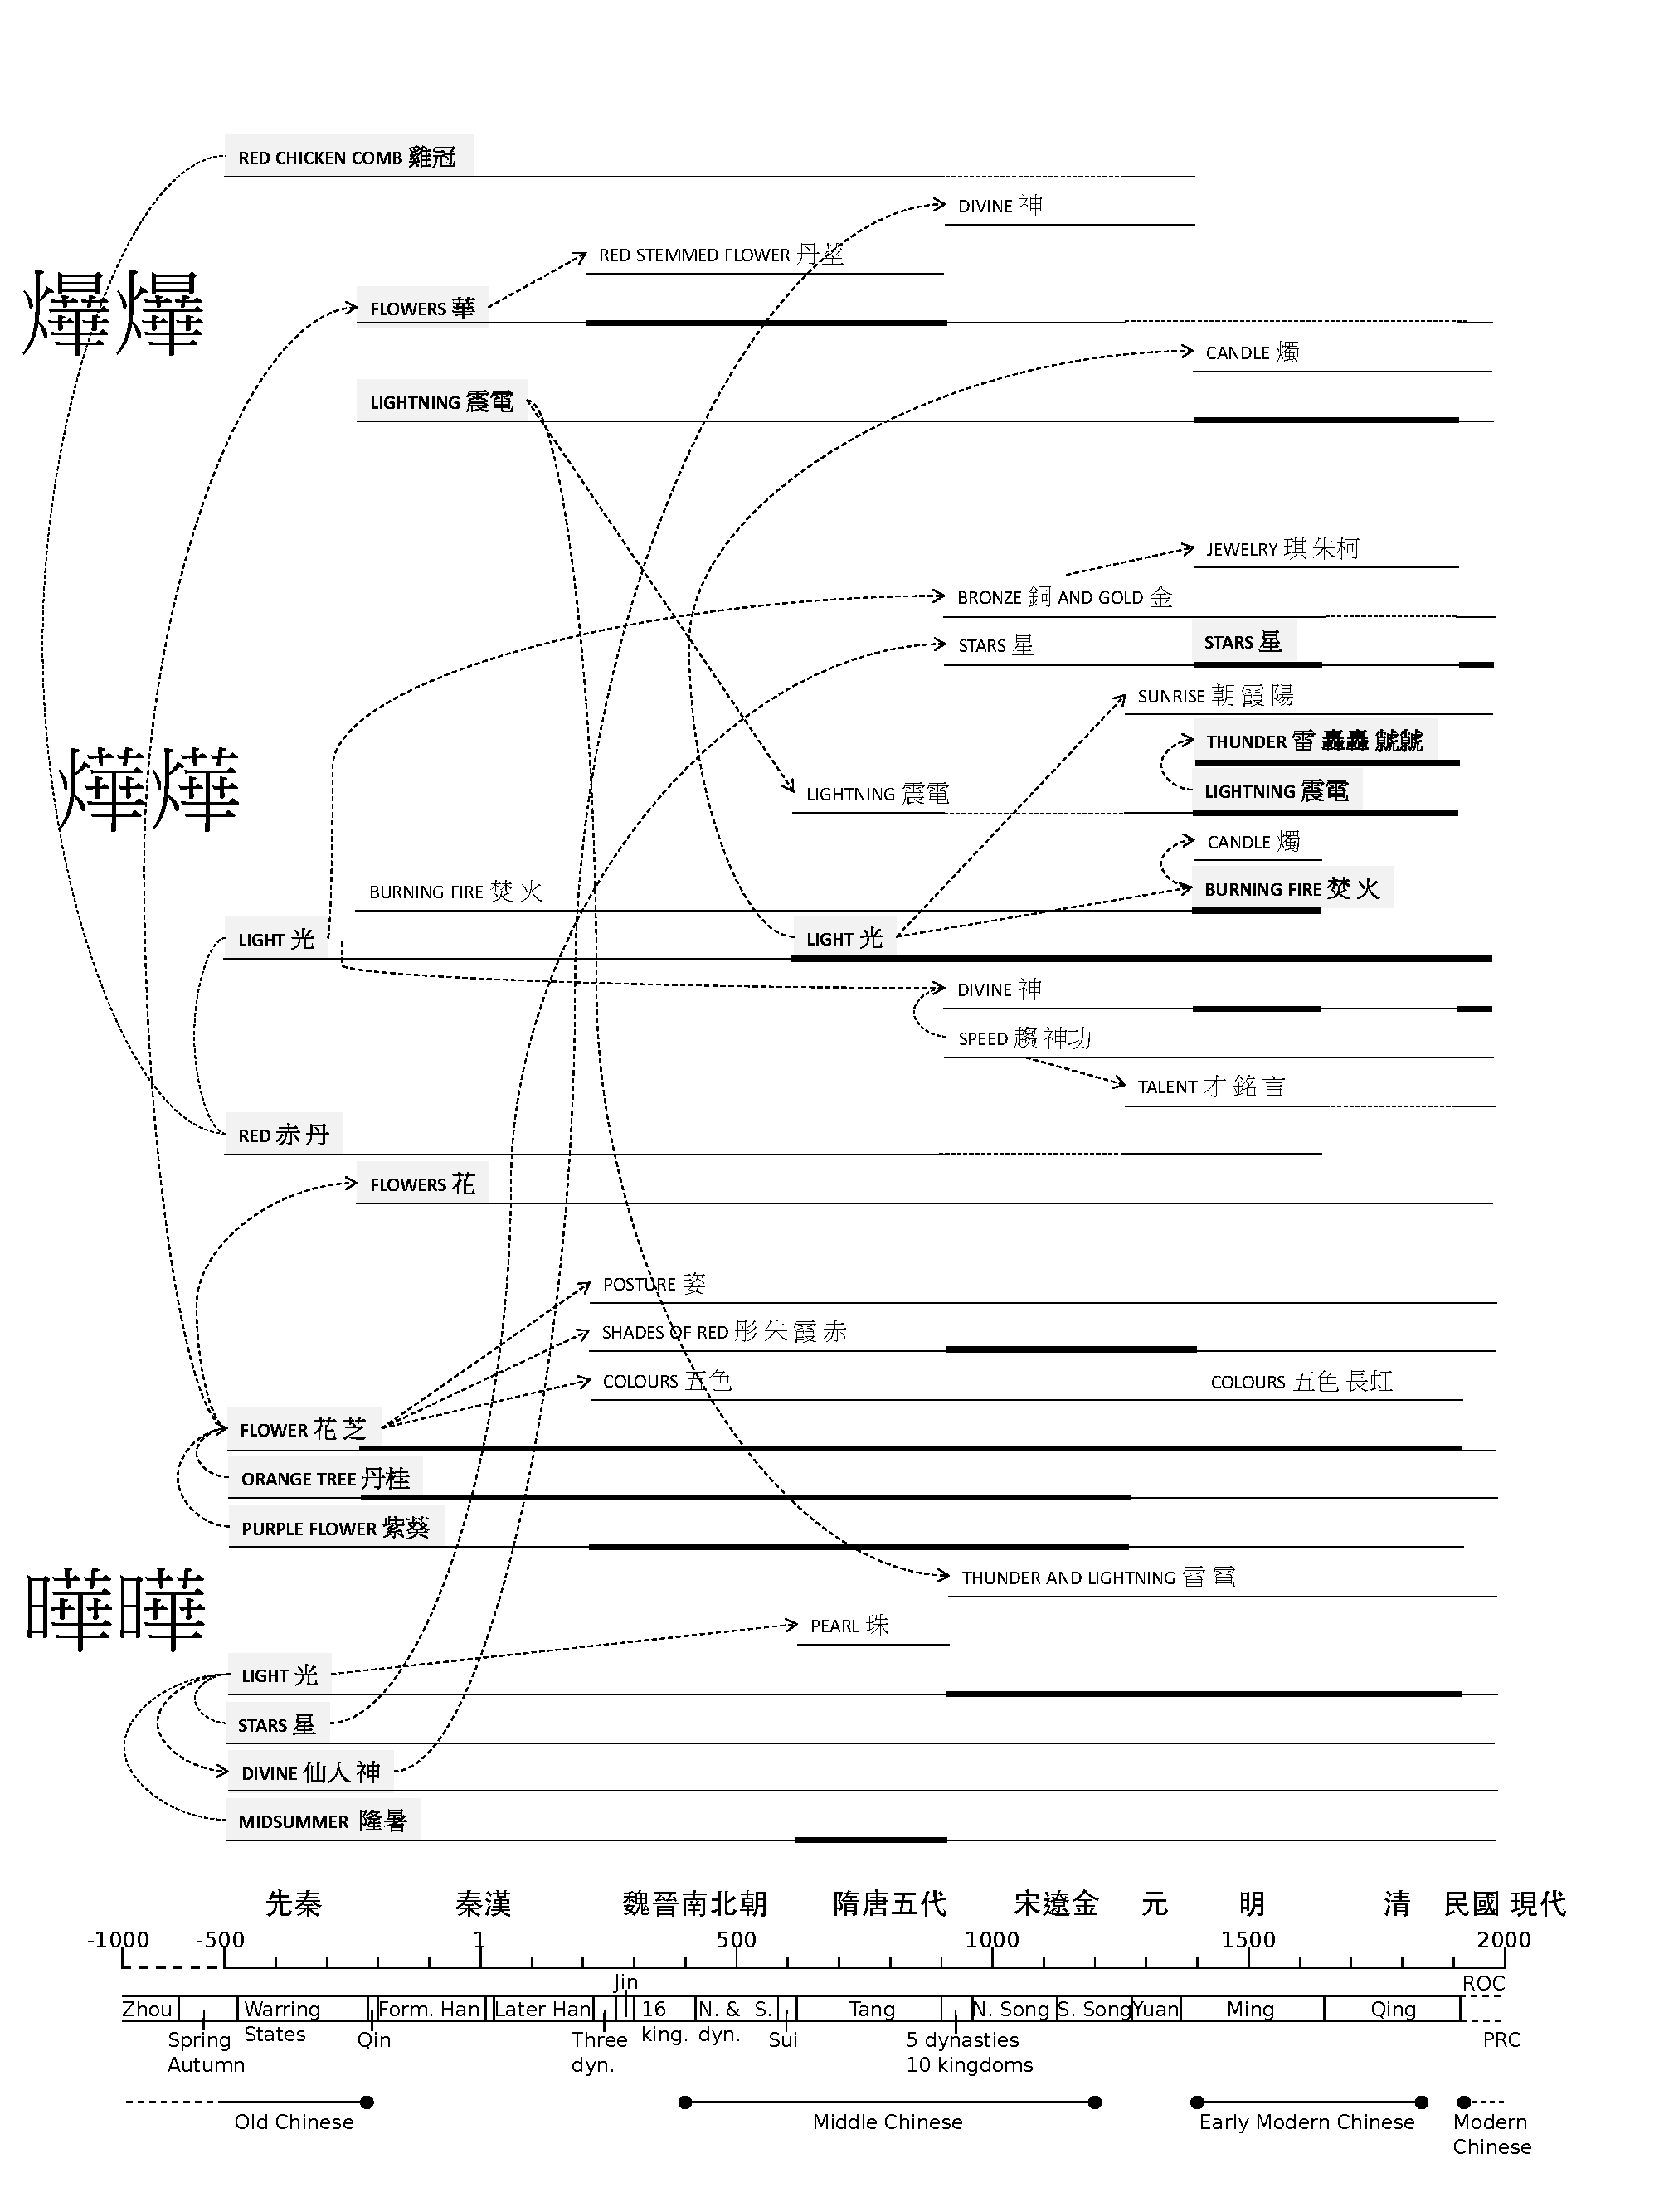
\includegraphics{ideos/yeye.pdf}
\caption{\label{fig:yeye}yeye 爗爗, yeye 燁燁 and yeye 曄曄}
\end{figure}

\section{Domains/ICMs and Image
Schemas}\label{domainsicms-and-image-schemas}

As we have argued in the sections above, we have successfully adopted
Kövecses's (2017) levels of metaphor theory to ideophones for mental
spaces (on a case-to-case basis) (Fauconnier 1994; Fauconnier \&
Sweetser 1996) and have in fact observed highly specialized frames when
these meanings became entrenched, as Akita (2012) suggested. Let us now
abstract it one level higher, to domains or ICMs (Lu 2006). This done by
taking the most prototypical meanings as they occur in the case studies
in a network and grouping them by their conceptual similarity.

\begin{figure}
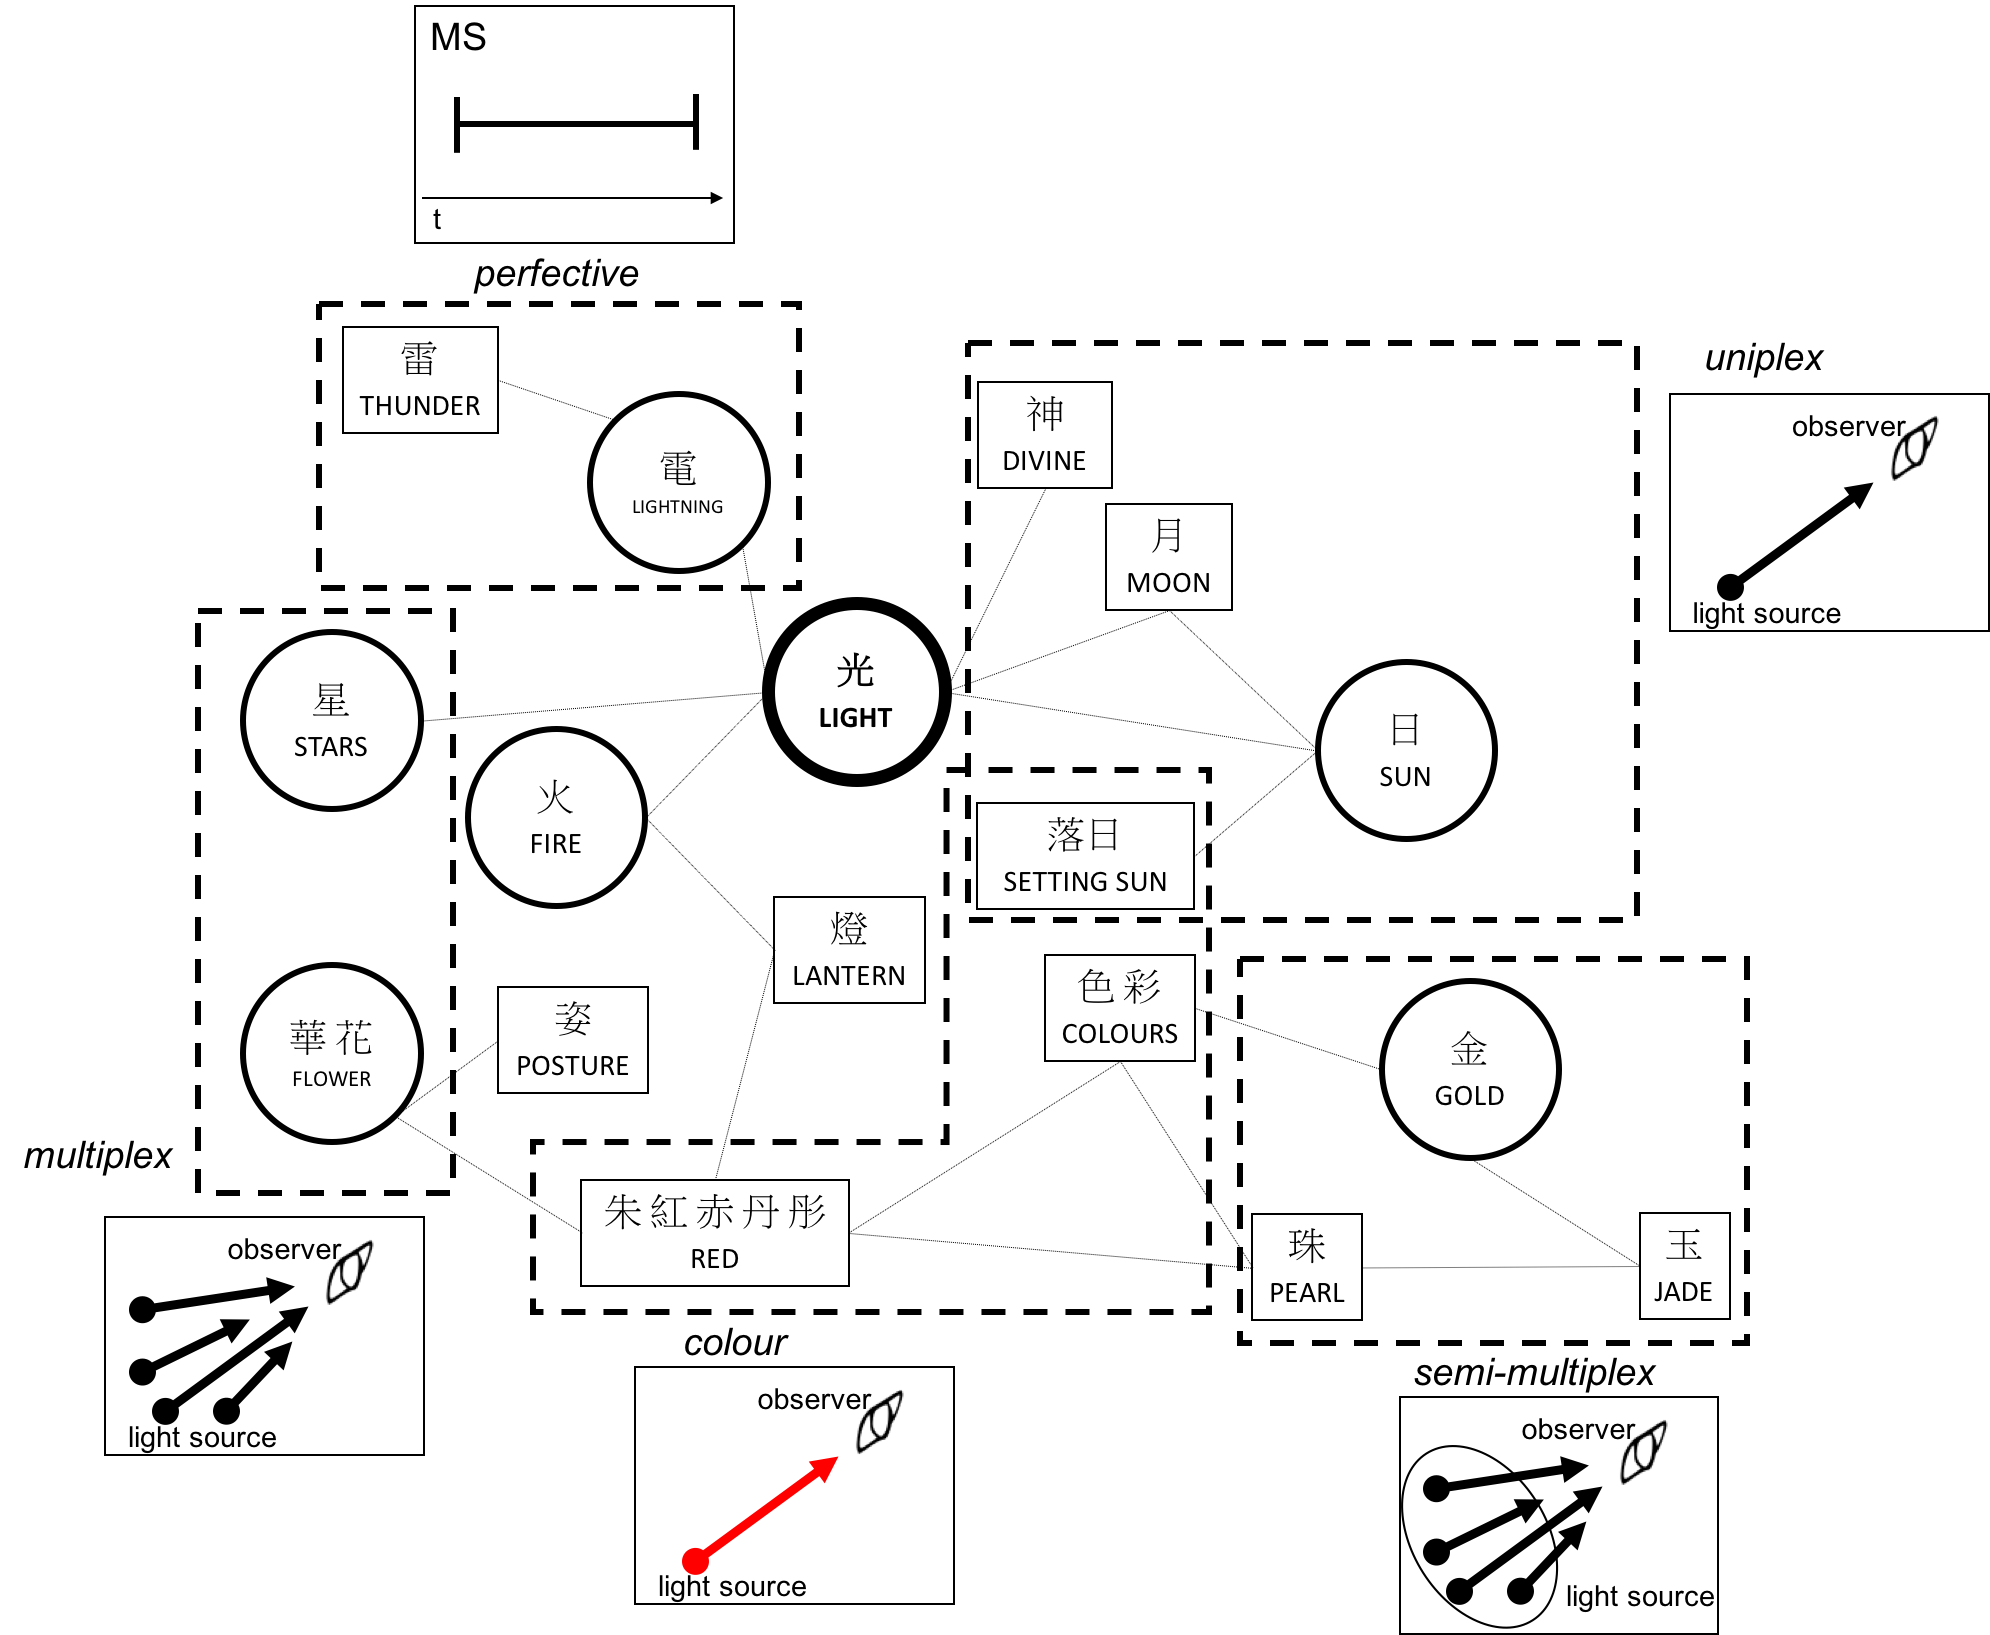
\includegraphics[width=27.64in]{ideos/domain2} \caption{Domains, ICMs and Image Schemas}\label{fig:domains}
\end{figure}

Figure 8 shows the result of such an exercise. When the different
frames, e.g.~the prototypical LIGHTNING frame (in a circle), and their
extended frames, e.g.~THUNDER (in a rectangle) are grouped like this, it
can be argued that the Domains or ICMs that bind these frames together
are different highlights of an underlying Image Schema. For the SUN
related frames, the uniplex domain shows how there is a single light
source, which reaches the observer. Light sources can also be multiplex
(Lakoff 1987; Talmy 2000), as in the case of STARS or FLOWERS, where it
is the distributed collectivity of light sources that depict the `LIGHT'
in this case. It can also be somewhere in between, as in the case of
metals like GOLD and related frames, where (presumably) it is different
smaller sparkling places within a bounded entity that depict the LIGHT.
For this reason, we have used the term semi-multiplex. Another aspect
that can be highlighted is the colours, with a strong preference for
RED. Since this is related to the reddish glow of the SUN, FIRE as well
as FLOWERS, it is motivated yet an unexpected productive domain of
extension. Finally, the boundedness or perfectivity (Langacker 2008:151,
156-157) of a LIGHT-related event may be highlighted as well, as in the
case of LIGHTNING and THUNDER.

\begin{figure}
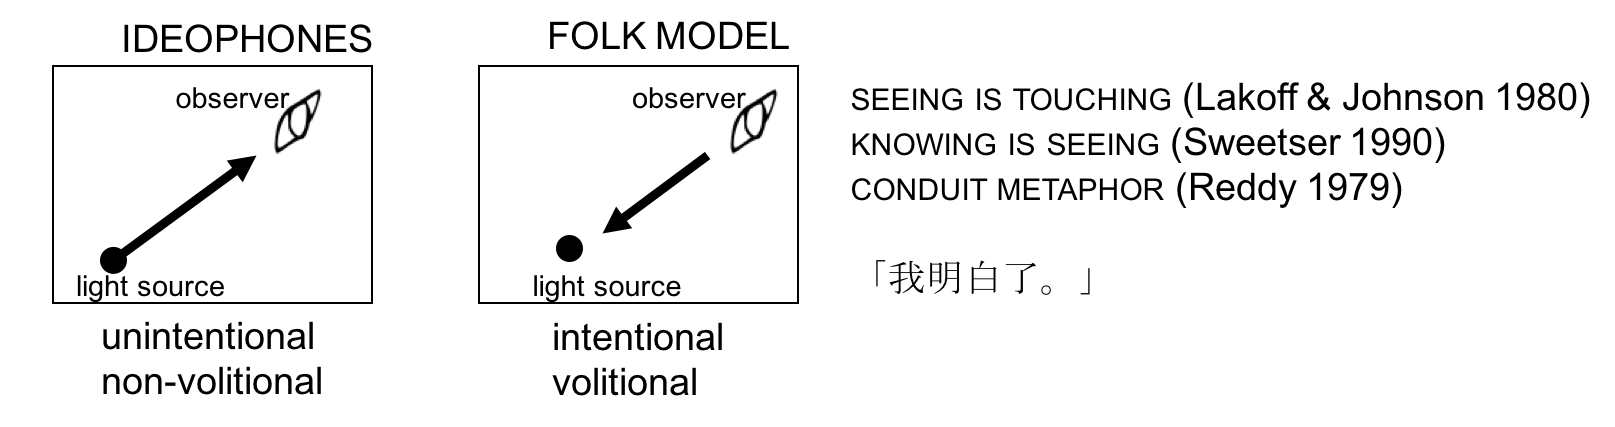
\includegraphics[width=22.43in]{ideos/folkmodel} \caption{Two different folk models}\label{fig:folk}
\end{figure}

Now, the reader may wonder why the most prototypical sense of LIGHT is
not included in any of these ICMs. Since in a way it is the result of
the overlapping meanings, it may be more useful to consider it a
proto-scene or Image Schema of `LIGHT FALLING INTO THE OBSERVER'S EYES'.
Notice how this differs from our usual way of understanding how light
works. From a scientific point-of-view (pun intended), a light source
emits beams of light that are caught by the observer's retina and
translated into electrical signals that are sent to the brain for
decoding, or that is how basic optics in physics works. However, our
folk model of light, at least as far as I have experienced it thus far,
thinks of SEEING and LOOKING AT as something volitional or intentional.
This is made clear by certain conceptual metaphors such as SEEING IS
TOUCHING (Lakoff \& Johnson 1980), KNOWING IS SEEING (Sweetser 1990) or
special instances of the CONDUIT metaphor (Reddy 1979), e.g.~the
Mandarin wo mingbai le 我明白了 `I understand \textless{} I clear
ASPECT'. In contrast to this way of thinking, there is at least one
important category where this folk model is reversed: ideophones. This
is not a surprise, because ideophones highlight the multimodal, mimetic
and performative nature of the experience, which is often unintentional.
The different models are presented in Figure 9, and capture the essense
of the highly abstract Image Schemas very well.

\section{Conclusion}\label{conclusion}

Using literary Chinese ideophones in the semantic domain of LIGHT as
case studies has revealed that the application of diachronic prototype
semantics in combination with the stratified `levels of metaphor'
approach to the study of ideophones is a fruitful venture. Regarding
prototypicality, it was shown that the meanings form interrelated
clusters of polysemy that are dynamic throughout time, with a clear
prototypical cores or prototypical bundles as a core, that developed
semantic extensions throughout time, see section 4.1 on yueyue. The
items investigated also seemed to influence one another, as the mutual
influence of the yaoyao case study displayed in section 4.2. In the next
section (4.3) huihui and zhuozhuo showed that type and token frequency
effects (Bybee 2001) also can play important roles in the semantic
development of these items. However, prototypicality is not only dynamic
between different meanings of an ideophonic item, it can also be among
different variants. The case study of yeye in section 4.4 showed that
some variants may be the most productive for a while, but others might
take over this role at one point. Prototypicality is thus transient.
These notions were all studied on the level of mental spaces and frames.
The interplay between dynamicity and stability is a direct consequence
from the flexibility mental space theory provides as a theory of online
meaning construction, and the opposite entrenching force of frames.
However, such an abstraction can be pushed even further. Domains or ICMs
were identified that each highlight something different of the embodied
Image Schema underlying most of these tokens. `LIGHT FALLING INTO THE
OBSERVER'S EYES' appears a good Image Schematic summary of what happens
when people use LIGHT ideophones to depict their experience. It does,
however, stand in stark contrast with the other folk model we have of
SEEING (cf.~section 5).

It is now also possible to generalize about the debate between vagueness
and polysemy. As mentioned in section 3.1, Akita (2012; 2013) mentions
that Mandarin SOUND ideophones are vague, while Japanese ones are
highly-specific. As our investigations above show, it is not a black and
white case. Take for example yeyeSUN in section 4.4, which has a
prototypical bundle of LIGHT, but also of FLOWER-related meanings. With
regards to polysemy at least these two big meanings will have to be
distinguished; with regards to vagueness, however, it can be argued that
the different readings of LIGHT, STARTS, the DIVINE and MIDSUMMER are
somewhat vague in the prototypical bundle of LIGHT. This resembles the
example of fruit discussed in section 3.2.

And now we turn back to the cognitive folk model we adopted in section
2.2 (repeated in example 12).

\[[\frac{sound}{writing}|MEANING]\]

We found considerable variation and dynamicity on the three poles of the
symbolic assembly. In the phonological pre-study, networks of word
families were found, as well as reanalysis in these networks. As for
meaning, this whole study has shown the flexibility of meanings from a
diachronic perspective. On the writing pole, the functional components
seem to play an important conceptual role as well: FIRE 火, LIGHT 光,
SUN 日, and METAL 金 all are prototypical frames identified in this
study (section 5), and that is exactly what distinguishes literary
Chinese ideophones from colloquial ones: the `radical support' and
motivation in the writing system, as Van Hoey as argued for
weather-related ideophones in Mandarin Chinese (2017).

A study as this one is not without limitations, however. A simple
example is the non-exhaustiveness of the lexical field that we were
aware of since the beginning. There probably exist other LIGHT
ideophones that we did not find because of the paradigmatic data
collection, driven by the database and the dictionary. For example, in
just the last few days, we have stumbled across yiyi 燡燡, yaoyao曜曜,
weiwei暐暐 and weiwei瑋瑋, all ideophones that would have complemented
this study. Yet, they would not have altered the conclusions
significantly, only enriched them. It shows also that research on this
topic is still only beginning and will grow incrementally as research is
undertaken. Summarizing, this curious set of phenomena warrants further
research, and the field is headed for a shining future, where dazzling
research will help us illuminate the splendid wonders of ideophones that
express LIGHT and other domains as well.

\section{References}\label{references}

Academia Sinica 中央研究院. 2015. Scripta Sinica Database (Hanji quanwen
ziliaoku jihua 漢籍全文資料庫計畫). Database. Scripta Sinica Database.
\url{http://hanchi.ihp.sinica.edu.tw/} (26 June, 2016). Akita, Kimi.
2012. Toward a frame-semantic definition of sound-symbolic words: A
collocational analysis of Japanese mimetics. Cognitive Linguistics
23(1). 67-90. Akita, Kimi. 2013. Constraints on the semantic extension
of onomatopoeia. Public Journal of Semiotics 13(1). 21-37. Baxter,
William Hubbard. 1992. A handbook of old Chinese phonology. (Trends in
Linguistics 64). Berlin\,; New York: Mouton de Gruyter. Baxter, William
Hubbard \& Laurent Sagart. 1998. Word formation in Old Chinese. In
Jerome Lee Packard (ed.), New approaches to Chinese word formation:
morphology, phonology and the lexicon in modern and ancient Chinese,
35-76. Berlin\,; New York: Mouton de Gruyter. Baxter, William Hubbard \&
Laurent Sagart. 2014. Old Chinese: a new reconstruction. Oxford\,; New
York: Oxford University Press. Baxter, William Hubbard \& Laurent
Sagart. 2015. Baxter-Sagart Old Chinese reconstruction (v. 13 october
2015).
\url{http://ocbaxtersagart.lsait.lsa.umich.edu/BaxterSagartOC2015-10-13.xlsx}.
Bybee, Joan L. 1985. Morphology: a study of the relation between meaning
and form. (Typological Studies in Language 9). Amsterdam: Benjamins.
Bybee, Joan L. 2001. Phonology and language use. (Cambridge Studies in
Linguistics). Cambridge, {[}England{]}\,; New York: Cambridge University
Press. Chang, Yufen. 2009. The phonology of ABB reduplication in
Taiwanese. In Yun Xiao (ed.), Proceedings of the 21st North American
Conference on Chinese Linguistics (NACCL-21): Vol. 1, 28-41. Smithfield,
Rhode Island: Bryant University. Dingemanse, Mark. 2011. The meaning and
use of ideophones in Siwu. Nijmegen: Radboud University Nijmegen
dissertation. Dingemanse, Mark. 2012. Advances in the cross-linguistic
study of ideophones. Language and Linguistics Compass 6(10). 654-672.
Dingemanse, Mark \& Kimi Akita. 2016. An inverse relation between
expressiveness and grammatical integration: On the morphosyntactic
typology of ideophones, with special reference to Japanese. Journal of
Linguistics. 1-32. \url{doi:10.1017/S002222671600030X}. Doke, Clement M.
1935. Bantu linguistic terminology. London\,; New York: Longmans, Green.
Fauconnier, Gilles. 1994. Mental spaces: aspects of meaning construction
in natural language. Cambridge\,; New York, NY, USA: Cambridge
University Press. Fauconnier, Gilles \& Eve Sweetser (eds.). 1996.
Spaces, worlds, and grammar. (Cognitive Theory of Language and Culture).
Chicago: University of Chicago Press. Geeraerts, Dirk. 1983. Prototype
theory and diachronic semantics: a case study. Indogermanische
Forschungen 88. 1-32. Geeraerts, Dirk. 1997. Diachronic prototype
semantics: a contribution to historical lexicology. (Oxford Studies in
Lexicography and Lexicology). Oxford\,: New York: Clarendon Press\,;
Oxford University Press. Geeraerts, Dirk. 2006a. Words and other
wonders: papers on lexical and semantic topics. (Cognitive Linguistics
Research 33). Berlin\,; New York: Mouton de Gruyter. Geeraerts, Dirk.
2006b. Idealist and empiricist tendencies in cognitive linguistics.
Words and other wonders: papers on lexical and semantic topics, 416-444.
(Cognitive Linguistics Research 33). Berlin\,; New York: Mouton de
Gruyter. Geeraerts, Dirk. 2010. Theories of Lexical Semantics. Oxford:
Oxford Univ. Press. Goddard, Cliff \& Anna Wierzbicka. 2014. Semantic
fieldwork and lexical universals. Studies in Language 38(1). 80-126.
Hampe, Beate \& Joseph E. Grady (eds.). 2005. From perception to
meaning: image schemas in cognitive linguistics. (Cognitive Linguistics
Research 29). Berlin\,; New York: Mouton de Gruyter. Haspelmath, Martin.
2007. Pre-established categories don't exist: Consequences for language
description and typology. Linguistic typology 11(1). 119-132.
Haspelmath, Martin. 2010a. Comparative concepts and descriptive
categories in crosslinguistic studies. Language 86(3). 663-687.
\url{doi:10.1353/lan.2010.0021}. Haspelmath, Martin. 2010b.
Framework-free grammatical theory. In Bernd Heine \& Heiko Narrog
(eds.), The Oxford handbook of linguistic analysis. (Oxford Handbooks in
Linguistics 341-366). Oxford\,; New York: Oxford University Press.
Hinton, Leanne, Johanna Nichols \& John J. Ohala (eds.). 1994. Sound
symbolism. Cambridge {[}England{]}\,; New York, NY: Cambridge University
Press. Huang, Chu-Ren \& Dingxu Shi (eds.). 2016. A reference grammar of
Chinese. Cambridge: Cambridge University Press. Iwasaki, Shoichi. 2015.
A multiple-grammar model of speakers' linguistic knowledge. Cognitive
Linguistics 26(2). \url{doi:10.1515/cog-2014-0101}.
\url{https://www.degruyter.com/view/j/cogl.2015.26.issue-2/cog-2014-0101/cog-2014-0101.xml}
(10 September, 2017). Johnson, Mark. 2005. The philosophical
significance of image schemas. In Beate Hampe \& Joseph E. Grady (eds.),
From perception to meaning: image schemas in cognitive linguistics,
15-33. (Cognitive Linguistics Research 29). Berlin\,; New York: Mouton
de Gruyter. Joseph, Brian D. 1997. On the linguistics of marginality:
The centrality of the periphery. Chicago Linguistic Society 33. 197-213.
Kövecses, Zoltán. 2017. Levels of metaphor. Cognitive Linguistics 28(2).
\url{doi:10.1515/cog-2016-0052}.
\url{http://www.degruyter.com/view/j/cogl.2017.28.issue-2/cog-2016-0052/cog-2016-0052.xml}
(14 October, 2017). Kroll, Paul W. 2015. A student's dictionary of
Classical and Medieval Chinese. (Handbook of Oriental Studies: Section 4
China 30). Leiden\,; Boston: Brill. Kwon, Nahyun. 2015. The natural
motivation of sound symbolism. Brisbane: University of Queensland PhD
dissertation. Kwon, Nahyun. 2017. Total reduplication in Japanese
ideophones: An exercise in Localized Canonical Typology. Glossa: a
journal of general linguistics 2(1). 40. \url{doi:10.5334/gjgl.267}.
Lakoff, George. 1987. Women, fire, and dangerous things: what categories
reveal about the mind. paperback ed., {[}Nachdr.{]}. Chicago: The Univ.
of Chicago Press. Lakoff, George \& Mark Johnson. 1980. Metaphors we
live by. Chicago: University of Chicago Press. Langacker, Ronald W.
1987. Foundations of Cognitive Grammar 1: Theoretical prerequisites.
Stanford, California: Stanford University Press. Langacker, Ronald W.
1988. An overview of Cognitive Grammar. In Brygida Rudzka-Ostyn (ed.),
Topics in cognitive linguistics, 3-48. (Amsterdam Studies in the Theory
and History of Linguistic Science v. 50). Amsterdam\,; Philadelphia: J.
Benjamins. Langacker, Ronald W. 1991a. Foundations of cognitive grammar
2: Descriptive application. Stanford, California: Stanford University
Press. Langacker, Ronald W. 1991b. Concept, image, and symbol: the
cognitive basis of grammar. 2nd ed., with a new preface. (Cognitive
Linguistics Research 1). Berlin\,; New York: Mouton de Gruyter.
Langacker, Ronald W. 2000. Grammar and conceptualization. (Cognitive
Linguistics Research 14). Berlin\,; New York: Mouton de Gruyter.
Langacker, Ronald W. 2008. Cognitive grammar: a basic introduction.
Oxford\,; New York: Oxford University Press. Lockwood, Gwilym \& Mark
Dingemanse. 2015. Iconicity in the lab: a review of behavioral,
developmental, and neuroimaging research into sound-symbolism. Frontiers
in Psychology 6(1246). 1-14. \url{doi:10.3389/fpsyg.2015.01246}. Lu
Chiarung 呂佳蓉. 2006. Giongo, gitaigo no hiyuteki kakuchō no shosō:
ninchi gengogaku to reikeiron no kanten kara. Kyōto: Kyōto University
PhD dissertation. Magnus, Margaret. 2001. What's in a word? Studies in
phonosemantics. Trondheim: Norwegian University of Sciente and
Technology (NTNU) PhD dissertation. Mok, Waiching Enid. 2001. Chinese
sound symbolism: A phonological perspective. Hawai'i: University of
Hawai'i PhD dissertation. Nuckolls, Janice. 2016. Rethinking
mono-sensory implicational approaches to ideophones in Pastaza Quichua.
Mimetics in Japanese and other languages in the world
(日本語と世界諸言語のオノマトペ). Tachikawa: NINJAL. Nuckolls, Janis B.
1996. Sounds like life: sound-symbolic grammar, performance, and
cognition in Pastaza Quechua. (Oxford Studies in Anthropological
Linguistics 2). New York: Oxford University Press. Nuckolls, Janis B.
1999. The case for sound symbolism. Annual Review of Anthropology.
225-252. Nuckolls, Janis B. 2001. Ideophones in Pastaza Quechua. In
Erhard Friedrich Karl Voeltz \& Christa Kilian-Hatz (eds.), Ideophones,
271-286. (Typological Studies in Language v. 44). Amsterdam\,;
Philadelphia: J. Benjamins. Nuckolls, Janis B. 2010. Lessons from a
Quechua strongwoman: ideophony, dialogue, and perspective. (First
Peoples). Tucson: University of Arizona Press. Nuckolls, Janis B. 2014.
Ideophones' challenges for typological linguistics: The case of Pastaza
Quichua. Pragmatics and Society 5(3). 355-383.
\url{doi:10.1075/ps.5.3.03nuc}. Nuckolls, Janis B., Tod D. Swanson,
Diana Shelton, Alexander Rice \& Sarah Hatton. 2017. Lexicography
in-your-face: The active semantics of Pastaza Quichua ideophones.
Canadian Journal of Linguistics/Revue canadienne de linguistique 62(02).
154-172. \url{doi:10.1017/cnj.2017.9}. Oakley, Todd. 2007. Image
schemas. In Dirk Geeraerts \& H. Cuyckens (eds.), The Oxford handbook of
cognitive linguistics, 214-235. (Oxford Handbooks). Oxford\,; New York:
Oxford University Press. Packard, Jerome Lee. 2001. The morphology of
Chinese: a linguistic and cognitive approach (Hanyu xingtaixue: Yuyan
renzhi yanjiufa汉语形态学\,: 语言认知硏究法). (Ed.) Shi Dingxu 石定栩.
Beijing: Waiyu jiaoxue yu yanjiu chubanshe. Reddy, Michael J. 1979. The
conduit metaphor: a case of frame conflict in our language about
language. In Andrew Ortony (ed.), Metaphor and thought, 284-324.
Cambridge: Cambridge Univ. Press. Rosch, Eleanor. 1975. Cognitive
representations of semantic categories. Journal of Experimental
Psychology: General 104(3). 192-233. Rosch, Eleanor \& Carolyn B.
Mervis. 1975. Family resemblances: Studies in the internal structure of
categories. Cognitive Psychology 7(4). 573-605. Sagart, Laurent. 1999.
The roots of old Chinese. (Amsterdam Studies in the Theory and History
of Linguistic Science Series 4, Current Issues in Linguistic Theory
184). Amsterdam: Benjamins. Sidhu, David M. \& Penny M. Pexman. 2017.
Five mechanisms of sound symbolic association. Psychonomic Bulletin \&
Review. \url{doi:10.3758/s13423-017-1361-1}.
\url{http://link.springer.com/10.3758/s13423-017-1361-1} (21 September,
2017). Sweetser, Eve. 1990. From etymology to pragmatics: metaphorical
and cultural aspects of semantic structure. Transferred to digital
print. (Cambridge Studies in Linguistics 54). Cambridge: Cambridge Univ.
Press. Talmy, Leonard. 2000. Toward a cognitive semantics: Volume 1.
(Language, Speech, and Communication). Cambridge, Mass: MIT Press.
Thompson, Arthur Lewis. 2017. Debunking phonaesthemes: The absence of
iconicity. CLS-MPI Iconicity Focus Group Workshop: Types of Iconicity in
Language Use, Development and Processing. Nijmegen: Max Planck Institute
for Psycholinguistics. Thompson, Sandra A. \& Paul J. Hopper. 2001.
Transitivity, clause structure, and argument structure: Evidence from
conversation. In Joan L. Bybee \& Paul J. Hopper (eds.), Frequency and
the emergence of linguistic structure, 27-60. (Typological Studies in
Language 45). Amsterdam: Benjamins. Tuggy, David. 1993. Ambiguity,
polysemy, and vagueness. In Dirk Geeraerts (ed.), Cognitive linguistics:
basic readings, 167-184. (Cognitive Linguistics Research 34). Berlin\,;
New York: Mouton de Gruyter. Tyler, Andrea \& Vyvyan Evans. 2003. The
semantics of English prepositions: Spatial scenes, embodied meaning, and
cognition. Cambridge\,; New York: Cambridge University Press. Van Hoey,
Thomas. 2015. Ideophones in Middle Chinese: a typological study of a
Tang dynasty poetic corpus. Leuven: KU Leuven Master thesis. Van Hoey,
Thomas. 2017. The thunder rolls: iconicity and ideophones in Chinese
meteorological expressions. CLS-MPI Iconicity Focus Group Workshop:
Types of Iconicity in Language Use, Development and Processing.
Nijmegen: Max Planck Institute for Psycholinguistics. Van Hoey, Thomas
\& Chiarung Lu. under review. A semantic map for ideophones: From an
implicational hierarchy to the spinning top model. Cognitive
Linguistics. Voeltz, Erhard Friedrich Karl \& Christa Kilian-Hatz
(eds.). 2001. Ideophones. (Typological Studies in Language v. 44).
Amsterdam\,; Philadelphia: J. Benjamins. Wierzbicka, Anna. 1992.
Defining emotion concepts. Cognitive science 16. 539-581.




\end{document}

